\section{Analysis Postfit Regions}\label{appsec-vh-analRegPosfit}
\addtocontents{toc}{\protect\setcounter{tocdepth}{1}}
\subsection{Resolved Postfit Regions}\label{appsec-vh-analRegResPosfit}
All regions in the resolved regime of the combined \vhbc\ analysis after the conditional fit to data of Section \ref{sec-fitFramework} are presented here, organised by increasing number of charged lepton channels (0L, 1L, 2L). The distributions indicate the pre-fit expectations of the sum of processes in dashed blue lines and highlight multiples (for visibility) of either the \vhb\ or \vhc\ signal distributions in red lines. The distribution variables presented, \gls{bdt}, \ptv, etc., correspond to the one used in the fit. Figures \ref{fig:plots_VHbb_OL_SR}, \ref{fig:plots_VHbb_1L_SR}, and \ref{fig:plots_VHbb_2L_SR} are the $BB$-tagged signal regions. The 2 $c$-tagged \glspl{sr} are displayed in Figures \ref{fig:plots_VHcc_OL_SR_2c}, \ref{fig:plots_VHcc_1L_SR_2c}, and \ref{fig:plots_VHcc_2L_SR_2c}. The 1 $c$-tagged \glspl{sr} are displayed in Figures \ref{fig:plots_VHcc_OL_SR_1c}, \ref{fig:plots_VHcc_1L_SR_1c}, and \ref{fig:plots_VHcc_2L_SR_1c}. \\

The different control regions presented can be grouped as:
\begin{itemize}
  \item The $BB$-tagged \highdr\ \glspl{cr} in Figures \ref{fig:plots_VHbb_OL_CRH}, \ref{fig:plots_VHbb_1L_CRH}, and \ref{fig:plots_VHbb_2L_CRH}.
  \item The $c$-tagged ($TN$, $TL$, and $TT$) \highdr\ \glspl{cr} in Figures \ref{fig:plots_VHcc_OL_CRH_2c_2J}, \ref{fig:plots_VHcc_OL_CRH_2c_3J}, \ref{fig:plots_VHcc_1L_CRH_2J}, \ref{fig:plots_VHcc_1L_CRH_3J}, \ref{fig:fig:plots_VHcc_2L_CRH_2J}, and \ref{fig:plots_VHcc_2L_CRH_3J}.
  \item The 1L $BB$-tagged \lowdr\ \glspl{cr} in Figure \ref{fig:plots_VHbb_1L_CRL}.
  \item The 1L and 2L $V+l$ \glspl{cr} ($LN$-tagged) in Figures \ref{fig:plots_VHcc_1L_LN} and \ref{fig:plots_VHcc_2L_LN}.
  \item The 0L and 1L top \glspl{cr} $BT$-tagged in Figures \ref{fig:plots_VHcc_OL_TopCR_2c} and \ref{fig:plots_VHcc_1L_TopCR}.
  \item The 2L top $e\mu$ \glspl{cr} with $\geq$ 1 $T$-tag in Figure \ref{fig:plots_VHcc_2L_topCRemu}.
\end{itemize}
  
\subsection{Boosted Postfit Regions}\label{appsec-vh-analRegBooPosfit}
This section presents the boosted regime regions after the conditional fit, with Figure \ref{fig:plots_VHbbBoost_OL} presenting the 0L regions, Figure \ref{fig:plots_VHbbBoost_1L} the 1L regions, and Figure \ref{fig:plots_VHbbBoost_2L_SR} the 2L regions. The distribution variables presented correspond to the ones used in the fit.

\clearpage

\begin{figure}[h!]
    \centering
    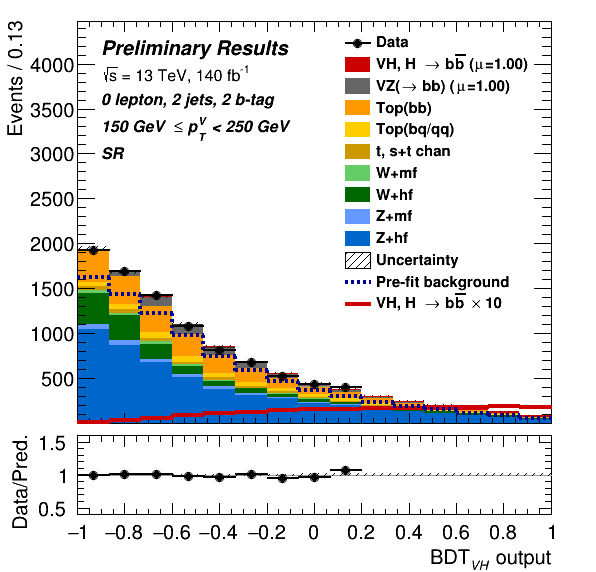
\includegraphics[width=0.32\textwidth]{Images/VH/postfit_VHbb/ZeroLep/Region_distmva_BMax250_BMin150_DSR_J2_TTypebb_T2_L0_Y6051_GlobalFit_conditionnal_mu1.pdf}
    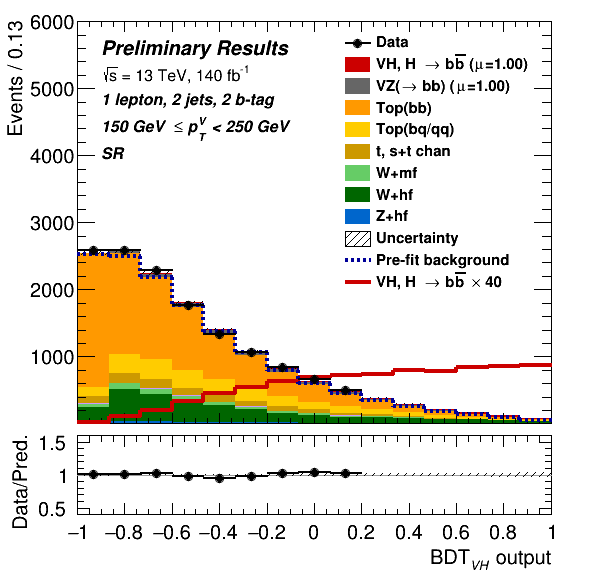
\includegraphics[width=0.32\textwidth]{ Images/VH/postfit_VHbb/OneLep/Region_distmva_BMax250_BMin150_DSR_J2_TTypebb_T2_L1_Y6051_GlobalFit_conditionnal_mu1.pdf}
    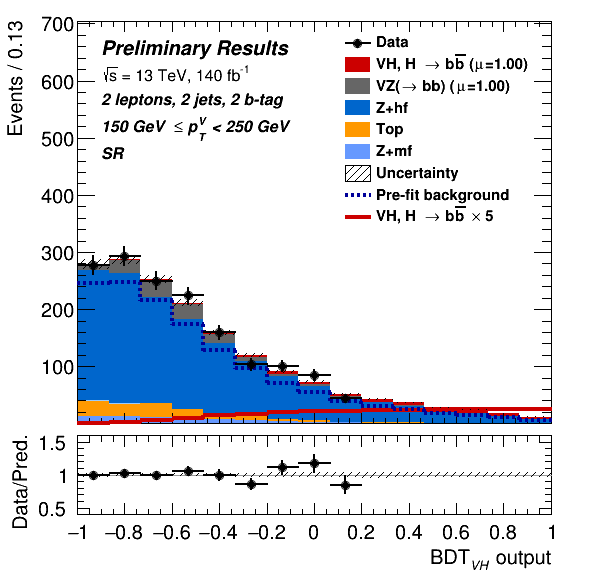
\includegraphics[width=0.32\textwidth]{ Images/VH/postfit_VHbb/TwoLep/Region_distmva_BMax250_BMin150_DSR_J2_TTypebb_T2_L2_Y6051_GlobalFit_conditionnal_mu1.pdf}
    \caption{The \vhb\ posfit conditional distribution in the 150 < \ptv\ < 250 GeV 2-jet signal region in the 0L (left), 1L (centre), and 2L (right).}
    \label{fig:plotsVHBSR_150pt_2J}
  \end{figure} 
  
  \begin{figure}[h!]
    \centering
    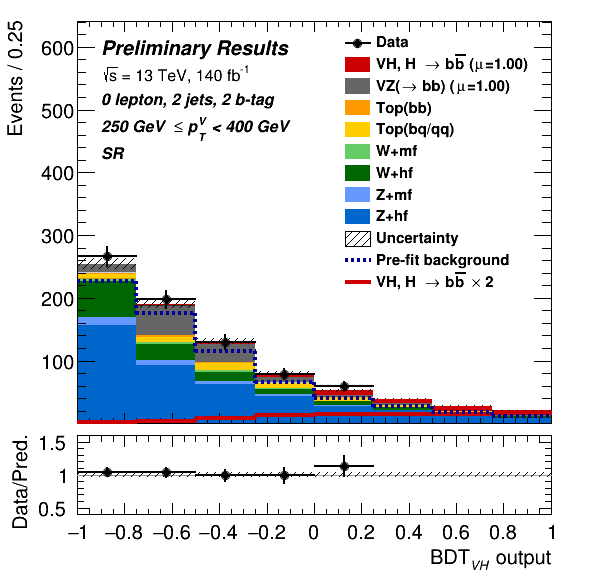
\includegraphics[width=0.32\textwidth]{Images/VH/postfit_VHbb/ZeroLep/Region_distmva_BMax400_BMin250_DSR_J2_TTypebb_T2_L0_Y6051_GlobalFit_conditionnal_mu1.pdf}
    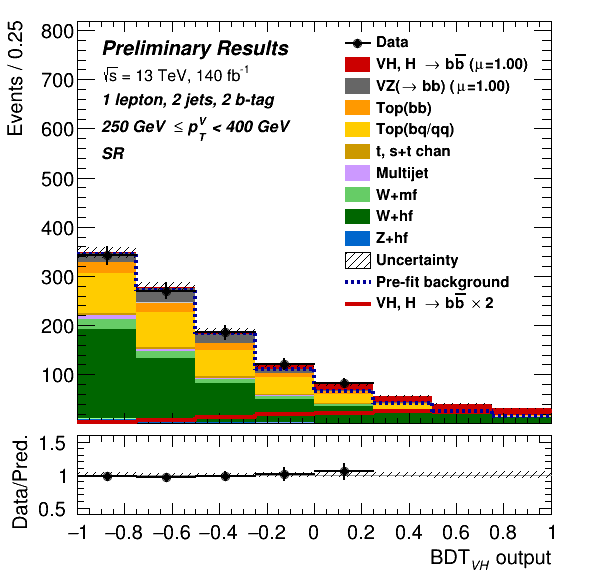
\includegraphics[width=0.32\textwidth]{ Images/VH/postfit_VHbb/OneLep/Region_distmva_BMax400_BMin250_DSR_J2_TTypebb_T2_L1_Y6051_GlobalFit_conditionnal_mu1.pdf}
    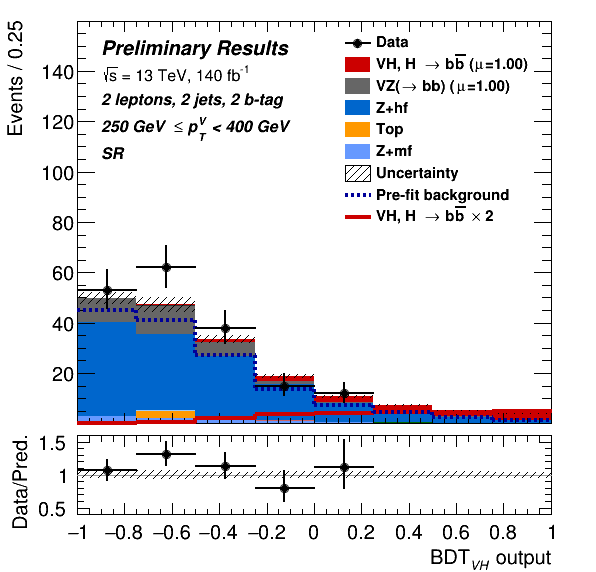
\includegraphics[width=0.32\textwidth]{ Images/VH/postfit_VHbb/TwoLep/Region_distmva_BMax400_BMin250_DSR_J2_TTypebb_T2_L2_Y6051_GlobalFit_conditionnal_mu1.pdf}
    \caption{The \vhb\ posfit conditional distribution in the 250 < \ptv\ < 400 GeV 2-jet signal region in the 0L (left), 1L (centre), and 2L (right).}
    \label{fig:plotsVHBSR_250pt_2J}
  \end{figure}
  
  \begin{figure}[h!]
    \centering
    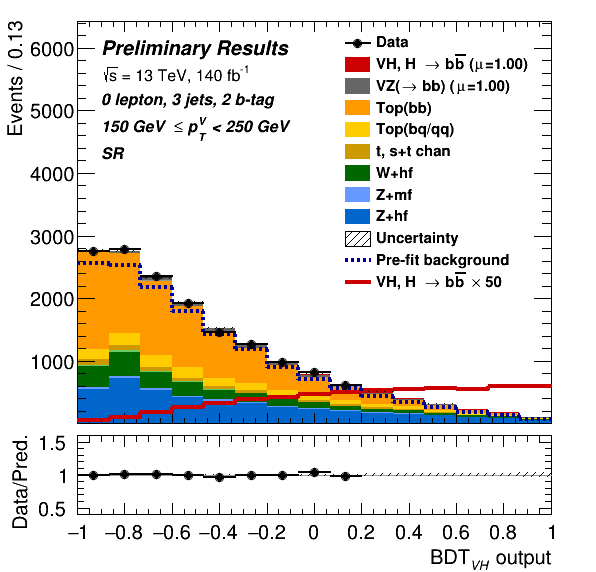
\includegraphics[width=0.32\textwidth]{Images/VH/postfit_VHbb/ZeroLep/Region_distmva_BMax250_BMin150_DSR_J3_TTypebb_T2_L0_Y6051_GlobalFit_conditionnal_mu1.pdf}
    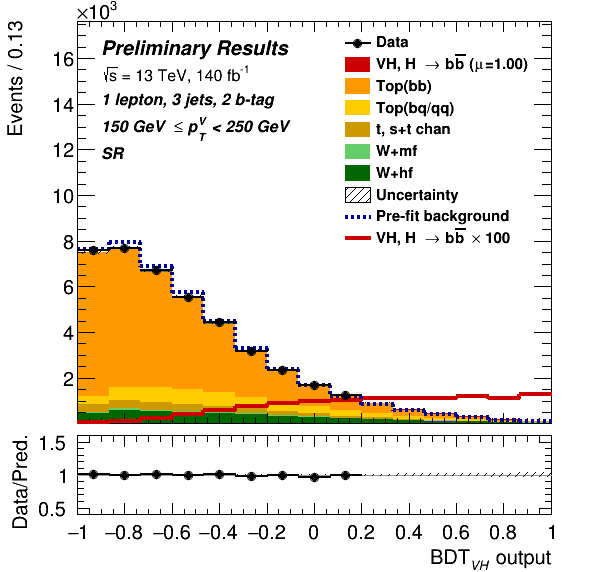
\includegraphics[width=0.32\textwidth]{Images/VH/postfit_VHbb/OneLep/Region_distmva_BMax250_BMin150_DSR_J3_TTypebb_T2_L1_Y6051_GlobalFit_conditionnal_mu1.pdf}
    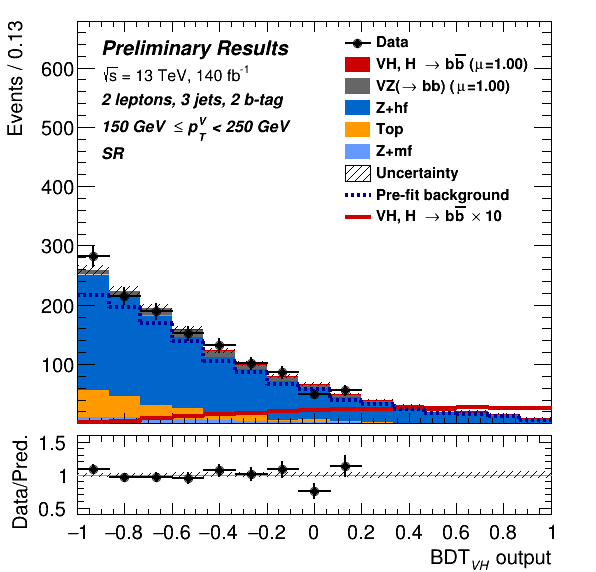
\includegraphics[width=0.32\textwidth]{Images/VH/postfit_VHbb/TwoLep/Region_distmva_BMax250_BMin150_DSR_J3_TTypebb_T2_L2_Y6051_GlobalFit_conditionnal_mu1.pdf}
    \caption{The \vhb\ posfit conditional distribution in the 150 < \ptv\ < 250 GeV 3-jet signal region in the 0L (left), 1L (centre), and 2L (right).}
    \label{fig:plotsVHBSR_150pt_3J}
  \end{figure} 
  
  \begin{figure}[h!]
    \centering
    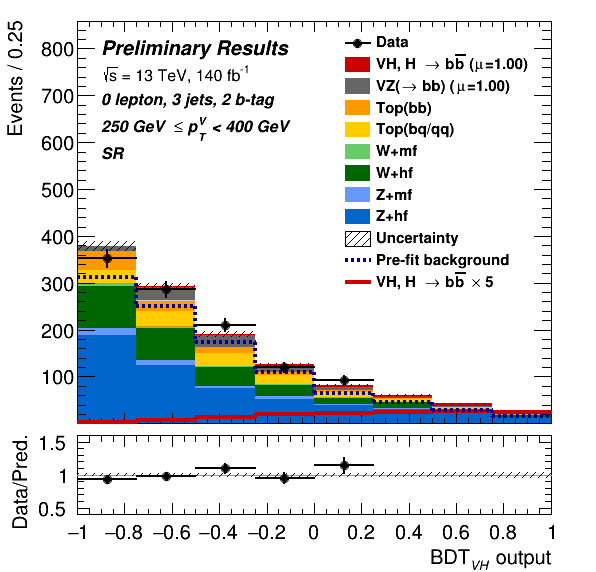
\includegraphics[width=0.32\textwidth]{Images/VH/postfit_VHbb/ZeroLep/Region_distmva_BMax400_BMin250_DSR_J3_TTypebb_T2_L0_Y6051_GlobalFit_conditionnal_mu1.pdf}
    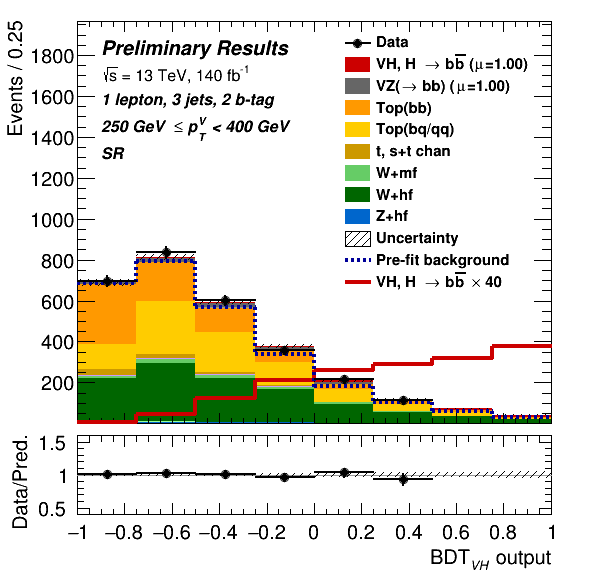
\includegraphics[width=0.32\textwidth]{ Images/VH/postfit_VHbb/OneLep/Region_distmva_BMax400_BMin250_DSR_J3_TTypebb_T2_L1_Y6051_GlobalFit_conditionnal_mu1.pdf}
    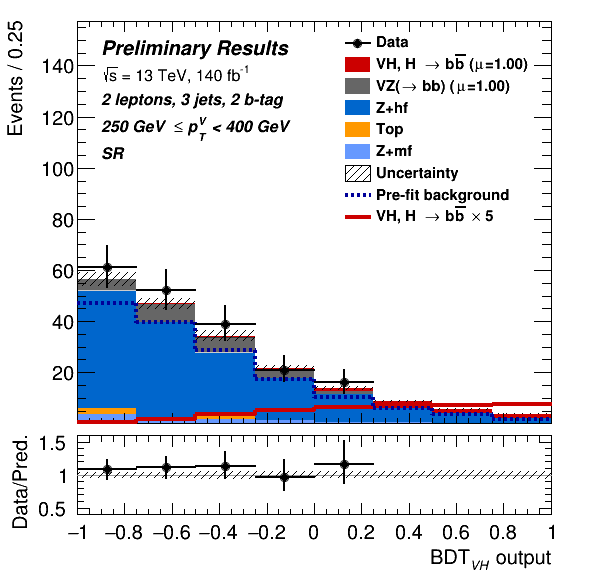
\includegraphics[width=0.32\textwidth]{ Images/VH/postfit_VHbb/TwoLep/Region_distmva_BMax400_BMin250_DSR_J3_TTypebb_T2_L2_Y6051_GlobalFit_conditionnal_mu1.pdf}
    \caption{The \vhb\ posfit conditional distribution in the 250 < \ptv\ < 400 GeV 3-jet signal region in the 0L (left), 1L (centre), and 2L (right).}
    \label{fig:plotsVHBSR_250pt_3J}
  \end{figure} 
  
  % 4J mid pTV
  \begin{figure}[h!]
    \centering
    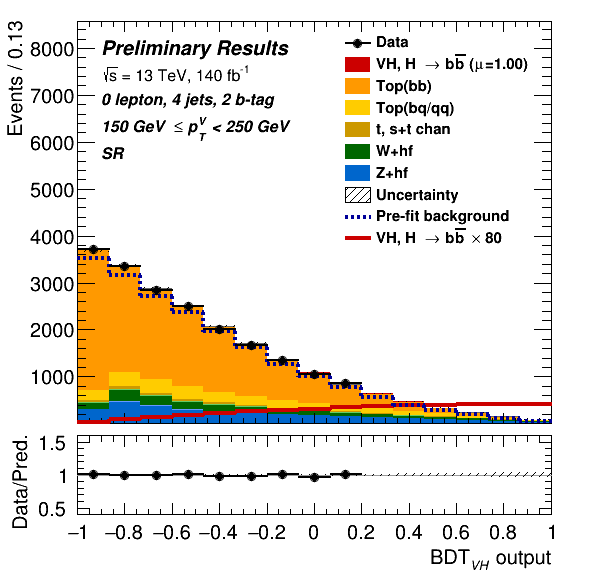
\includegraphics[width=0.24\textwidth]{Images/VH/postfit_VHbb/ZeroLep/Region_distmva_BMax250_BMin150_DSR_J4_TTypebb_T2_L0_Y6051_GlobalFit_conditionnal_mu1.pdf}
    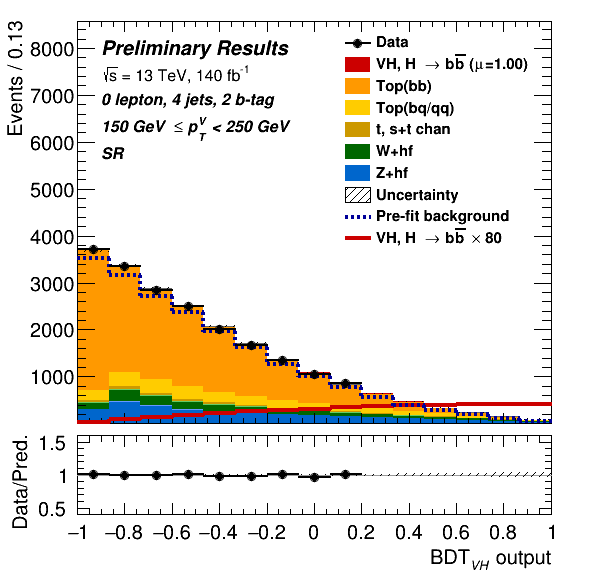
\includegraphics[width=0.24\textwidth]{Images/VH/postfit_VHbb/ZeroLep/Region_distmva_BMax250_BMin150_DSR_J4_TTypebb_T2_L0_Y6051_GlobalFit_conditionnal_mu1.pdf}
    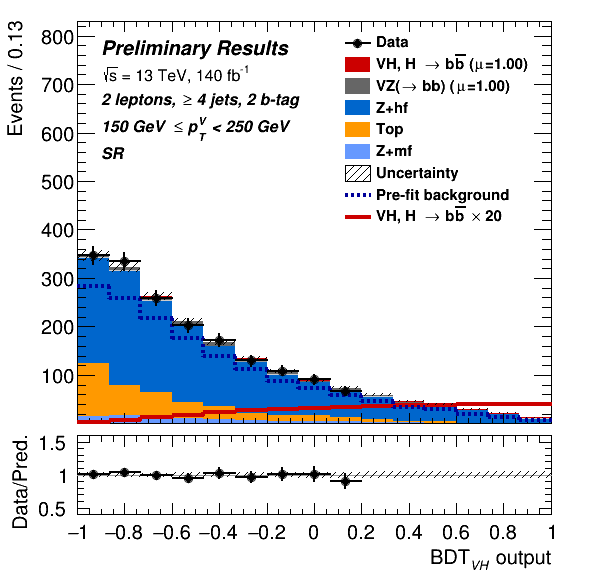
\includegraphics[width=0.24\textwidth]{ Images/VH/postfit_VHbb/TwoLep/Region_distmva_BMax250_BMin150_DSR_J4_TTypebb_incJet1_T2_L2_Y6051_GlobalFit_conditionnal_mu1.pdf}
    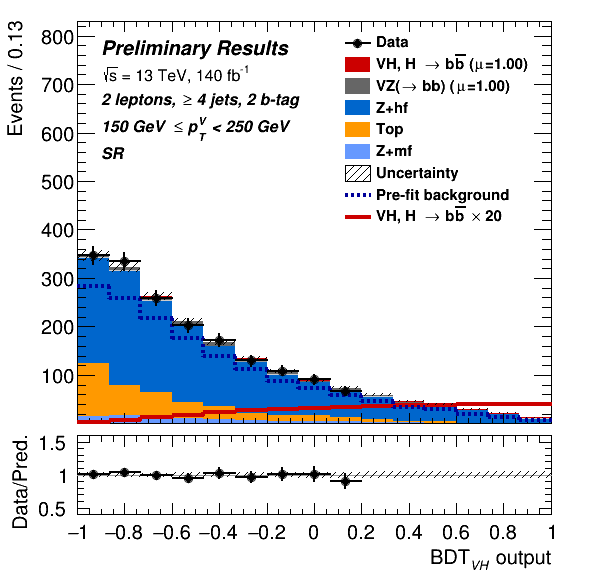
\includegraphics[width=0.24\textwidth]{ Images/VH/postfit_VHbb/TwoLep/Region_distmva_BMax250_BMin150_DSR_J4_TTypebb_incJet1_T2_L2_Y6051_GlobalFit_conditionnal_mu1.pdf}
    \caption{The \vhb\ posfit conditional distribution in the 150 < \ptv\ < 250 GeV 4-jet (4p-jet) signal region in the 0L (2 left) and 2L (2 right).}
    \label{fig:plotsVHBSR_150pt_4J}
  \end{figure} 
  
  \begin{figure}[h!]
    \centering
    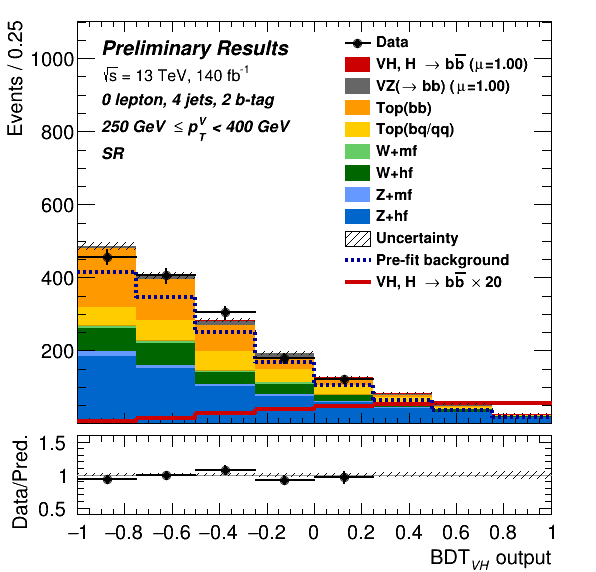
\includegraphics[width=0.24\textwidth]{Images/VH/postfit_VHbb/ZeroLep/Region_distmva_BMax400_BMin250_DSR_J4_TTypebb_T2_L0_Y6051_GlobalFit_conditionnal_mu1.pdf}
    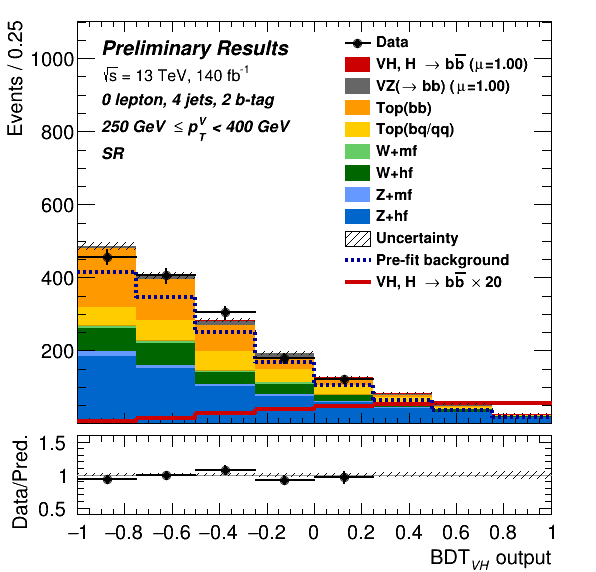
\includegraphics[width=0.24\textwidth]{Images/VH/postfit_VHbb/ZeroLep/Region_distmva_BMax400_BMin250_DSR_J4_TTypebb_T2_L0_Y6051_GlobalFit_conditionnal_mu1.pdf}
    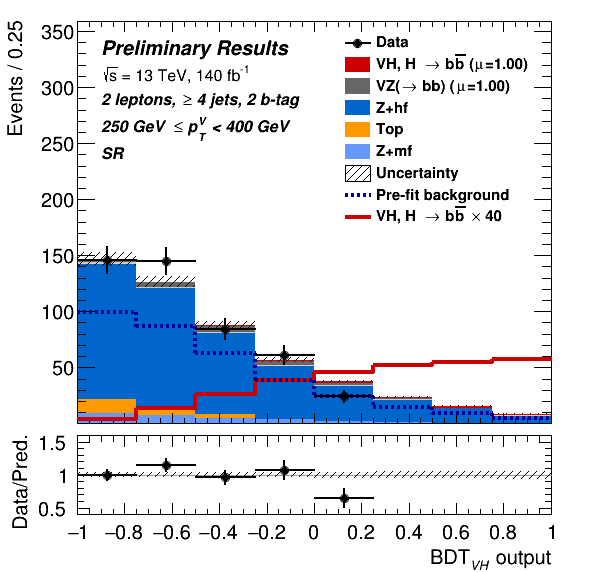
\includegraphics[width=0.24\textwidth]{ Images/VH/postfit_VHbb/TwoLep/Region_distmva_BMax400_BMin250_DSR_J4_TTypebb_incJet1_T2_L2_Y6051_GlobalFit_conditionnal_mu1.pdf}
    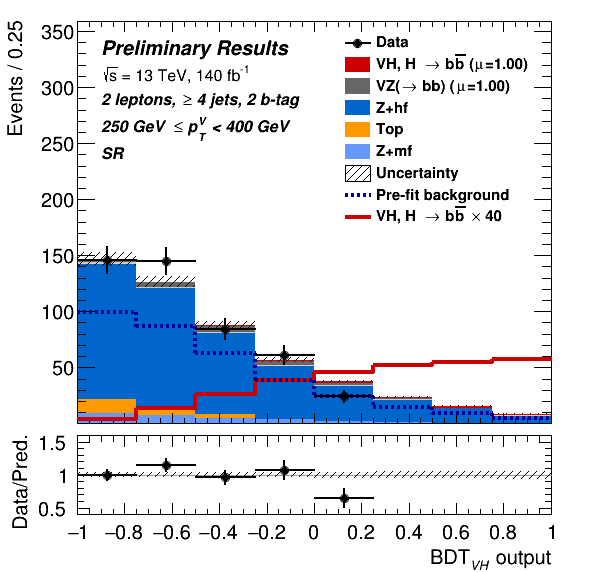
\includegraphics[width=0.24\textwidth]{ Images/VH/postfit_VHbb/TwoLep/Region_distmva_BMax400_BMin250_DSR_J4_TTypebb_incJet1_T2_L2_Y6051_GlobalFit_conditionnal_mu1.pdf}
    \caption{The \vhb\ posfit conditional distribution in the 150 < \ptv\ < 250 GeV 4-jet (4p-jet) signal region in the 0L (2 left) and 2L (2 right).}
    \label{fig:plotsVHBSR_250pt_4J}
  \end{figure} 
  
  % low pTV VHbb
  \begin{figure}[h!]
    \centering
    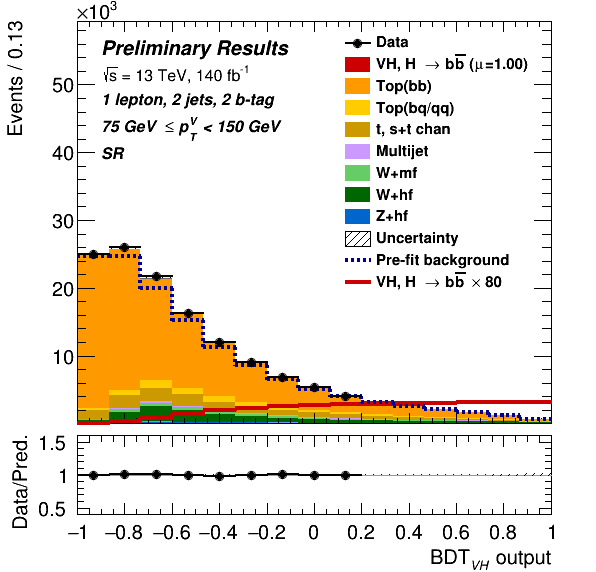
\includegraphics[width=0.32\textwidth]{Images/VH/postfit_VHbb/OneLep/Region_distmva_BMax150_BMin75_DSR_J2_TTypebb_T2_L1_Y6051_GlobalFit_conditionnal_mu1.pdf}
    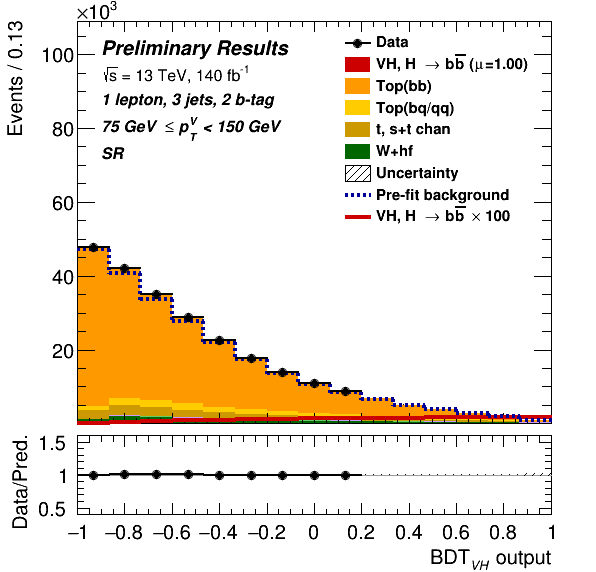
\includegraphics[width=0.32\textwidth]{Images/VH/postfit_VHbb/OneLep/Region_distmva_BMax150_BMin75_DSR_J3_TTypebb_T2_L1_Y6051_GlobalFit_conditionnal_mu1.pdf}
    \caption{The 1L \vhb\ posfit conditional distribution in the 75 < \ptv\ < 150 GeV 2-jet (left) and 3-jet (right) signal regions.}
    \label{fig:plotsVHBSR_75pt_1L}
  \end{figure} 
  
  \begin{figure}[h!]
    \centering
    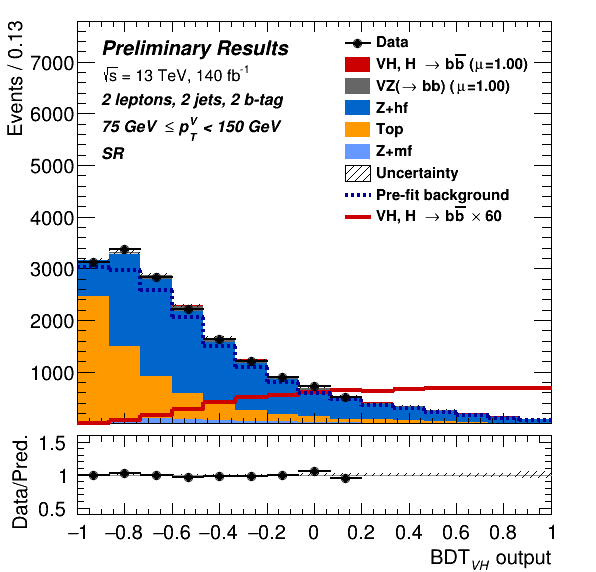
\includegraphics[width=0.32\textwidth]{Images/VH/postfit_VHbb/TwoLep/Region_distmva_BMax150_BMin75_DSR_J2_TTypebb_T2_L2_Y6051_GlobalFit_conditionnal_mu1.pdf}
    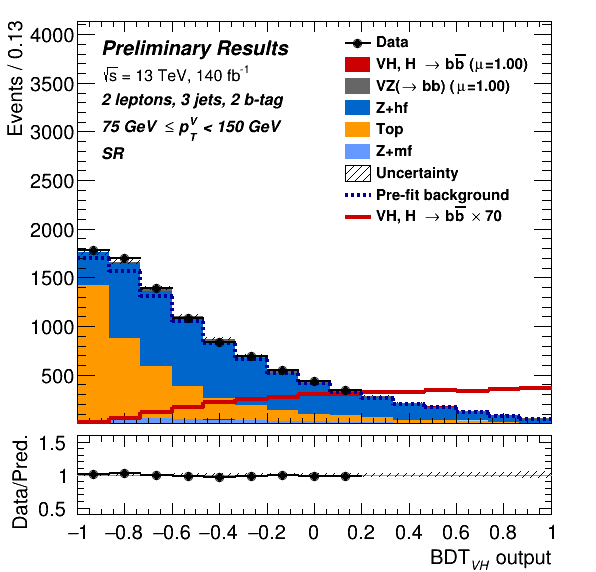
\includegraphics[width=0.32\textwidth]{Images/VH/postfit_VHbb/TwoLep/Region_distmva_BMax150_BMin75_DSR_J3_TTypebb_T2_L2_Y6051_GlobalFit_conditionnal_mu1.pdf}
    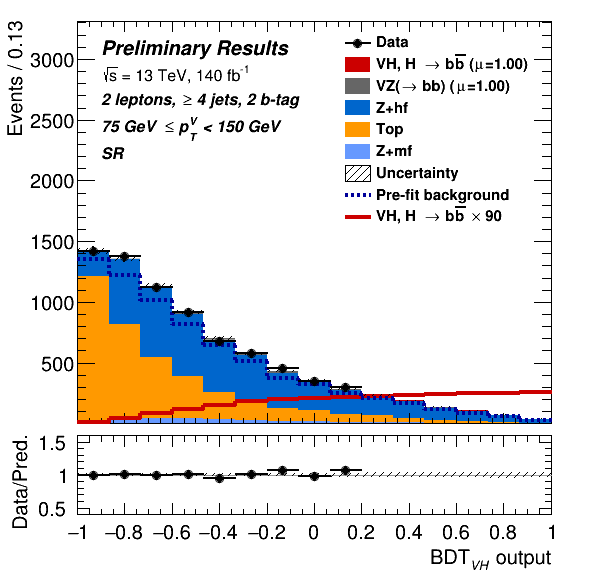
\includegraphics[width=0.32\textwidth]{Images/VH/postfit_VHbb/TwoLep/Region_distmva_BMax150_BMin75_DSR_J4_TTypebb_incJet1_T2_L2_Y6051_GlobalFit_conditionnal_mu1.pdf}
    \caption{The 2L \vhb\ posfit conditional distribution in the 75 < \ptv\ < 150 GeV 2-jet (left), 3-jet (centre) and 4p-jet (right) signal regions.}
    \label{fig:plotsVHBSR_75pt_2L}
  \end{figure} 
  
  %\begin{figure}[h!]
  %  \includegraphics[width=0.32\textwidth]{Images/VH/postfit_VHbb/ZeroLep/}
  %  \includegraphics[width=0.32\textwidth]{Images/VH/postfit_VHbb/OneLep/}
  %  \includegraphics[width=0.32\textwidth]{Images/VH/postfit_VHbb/TwoLep/}
  %  \caption{}
  %  \label{fig:plots}
  %\end{figure} 


 % ---


\begin{figure}[h!]
    \centering
    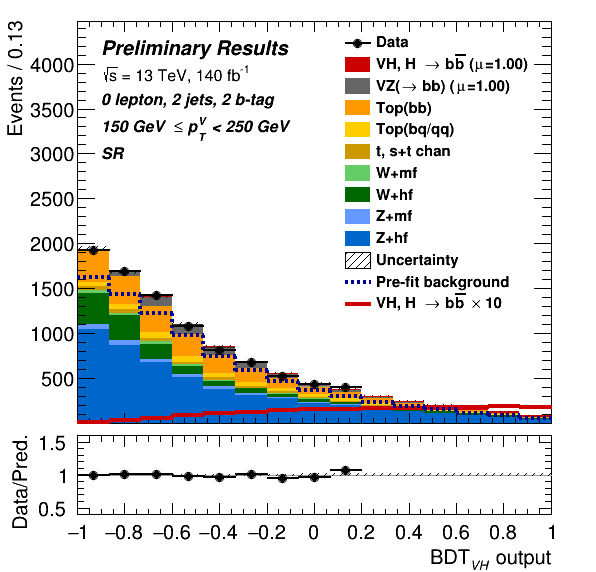
\includegraphics[width=0.32\textwidth]{Images/VH/postfit_VHbb/ZeroLep/Region_distmva_BMax250_BMin150_DSR_J2_TTypebb_T2_L0_Y6051_GlobalFit_conditionnal_mu1.pdf}
    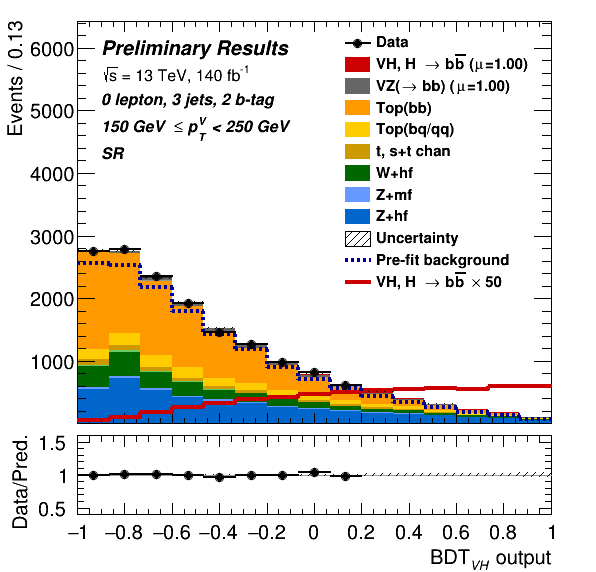
\includegraphics[width=0.32\textwidth]{Images/VH/postfit_VHbb/ZeroLep/Region_distmva_BMax250_BMin150_DSR_J3_TTypebb_T2_L0_Y6051_GlobalFit_conditionnal_mu1.pdf}
    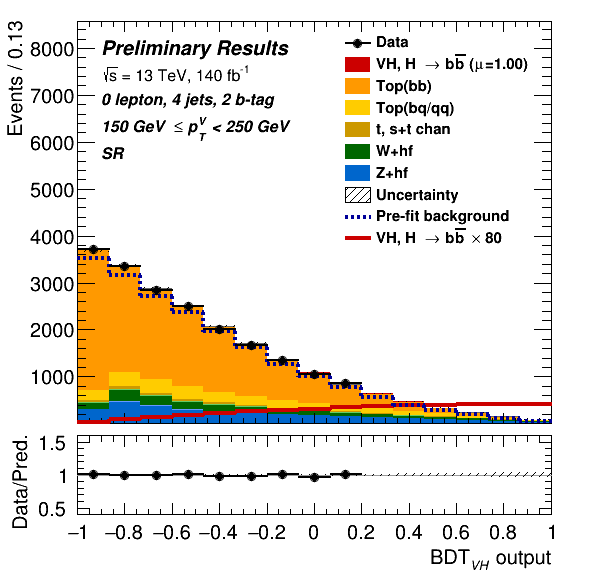
\includegraphics[width=0.32\textwidth]{Images/VH/postfit_VHbb/ZeroLep/Region_distmva_BMax250_BMin150_DSR_J4_TTypebb_T2_L0_Y6051_GlobalFit_conditionnal_mu1.pdf}
    \caption{The 0L posfit conditional distribution in the $BB$-tag, 150 < \ptv\ < 250 GeV, 2-jet(left), 3-jet (centre), and 4-jet (right) signal regions.}
    \label{fig:plotsVHBSR_150pt_0L}
\end{figure} 

\begin{figure}[h!]
    \centering
    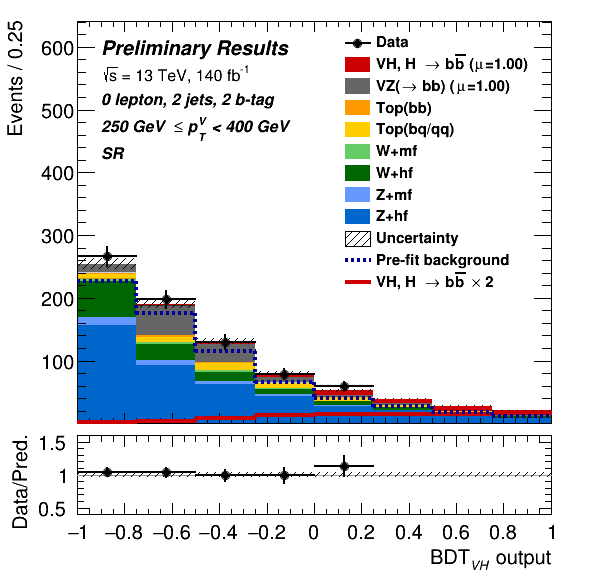
\includegraphics[width=0.32\textwidth]{Images/VH/postfit_VHbb/ZeroLep/Region_distmva_BMax400_BMin250_DSR_J2_TTypebb_T2_L0_Y6051_GlobalFit_conditionnal_mu1.pdf}
    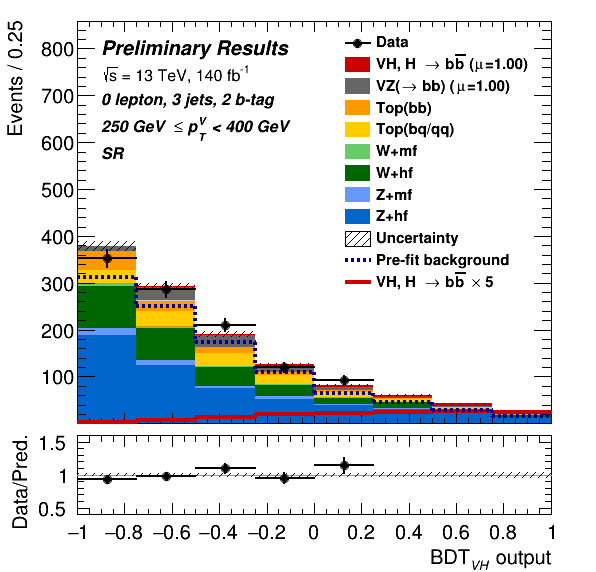
\includegraphics[width=0.32\textwidth]{Images/VH/postfit_VHbb/ZeroLep/Region_distmva_BMax400_BMin250_DSR_J3_TTypebb_T2_L0_Y6051_GlobalFit_conditionnal_mu1.pdf}
    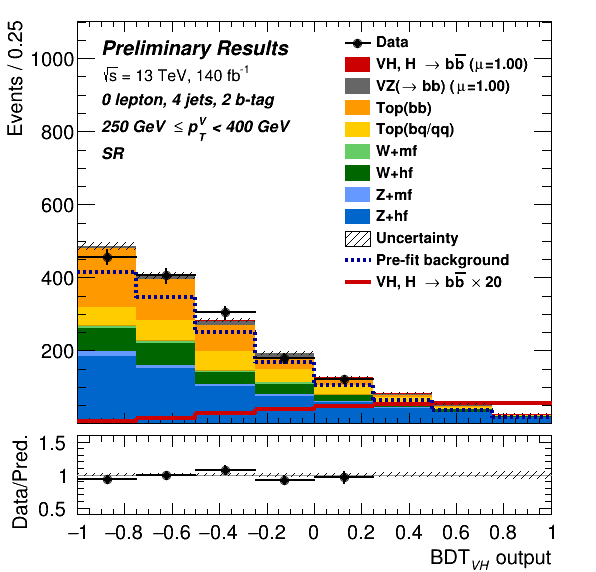
\includegraphics[width=0.32\textwidth]{Images/VH/postfit_VHbb/ZeroLep/Region_distmva_BMax400_BMin250_DSR_J4_TTypebb_T2_L0_Y6051_GlobalFit_conditionnal_mu1.pdf}
    \caption{The 0L posfit conditional distribution in the $BB$-tag, 250 < \ptv\ < 400 GeV, 2-jet(left), 3-jet (centre), and 4-jet (right) signal regions.}
    \label{fig:plotsVHBSR_250pt_0L}
\end{figure} 

\begin{figure}[h!]
    \centering
    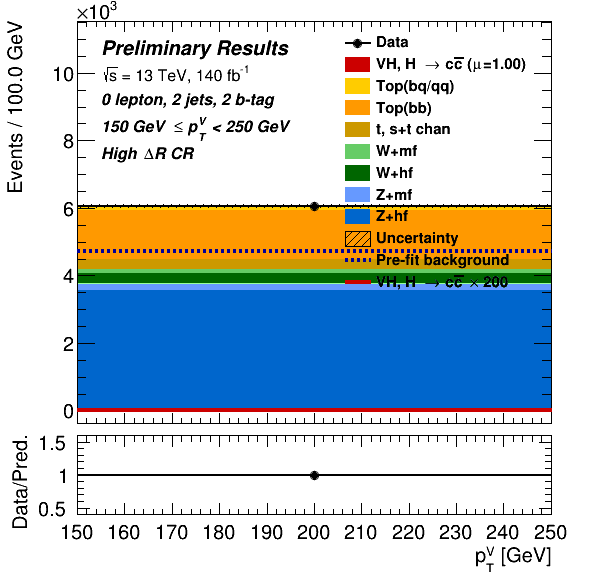
\includegraphics[width=0.32\textwidth]{Images/VH/postfit_VHbb/ZeroLep/Region_distpTV_BMax250_BMin150_DCRHigh_J2_TTypebb_T2_L0_Y6051_GlobalFit_conditionnal_mu1.pdf}
    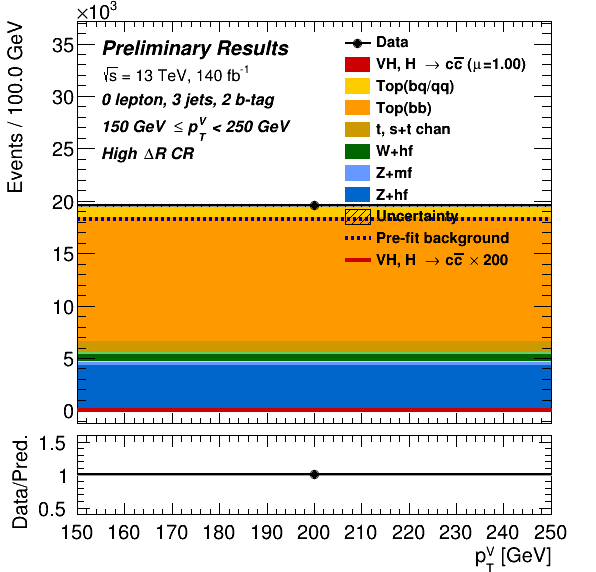
\includegraphics[width=0.32\textwidth]{Images/VH/postfit_VHbb/ZeroLep/Region_distpTV_BMax250_BMin150_DCRHigh_J3_TTypebb_T2_L0_Y6051_GlobalFit_conditionnal_mu1.pdf}
    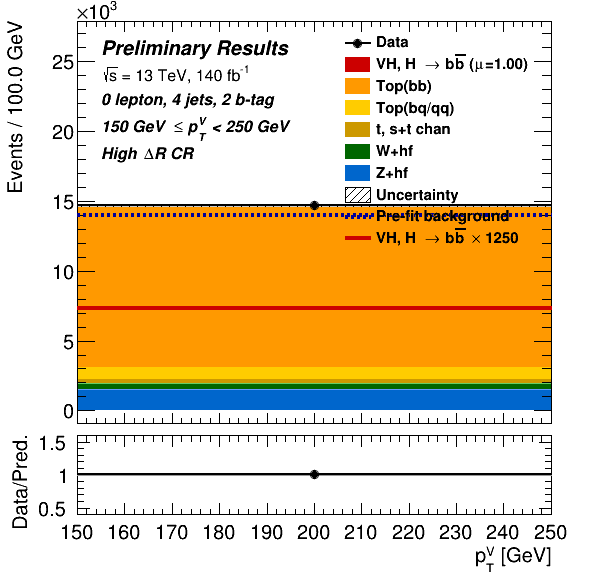
\includegraphics[width=0.32\textwidth]{Images/VH/postfit_VHbb/ZeroLep/Region_distpTV_BMax250_BMin150_DCRHigh_J4_TTypebb_T2_L0_Y6051_GlobalFit_conditionnal_mu1.pdf}
    \caption{The 0L posfit conditional distribution in the $BB$-tag, 150 < \ptv\ < 250 GeV 2-jet(left), 3-jet (centre), and 4-jet (right) signal regions.}
    \label{fig:plotsVHBSR_150pt_0L}
\end{figure} 


Region_distpTV_BMax250_BMin150_DCRHigh_J2_TTypebb_T2_L0_Y6051_GlobalFit_conditionnal_mu1.pdf
Region_distpTV_BMax250_BMin150_DCRHigh_J3_TTypebb_T2_L0_Y6051_GlobalFit_conditionnal_mu1.pdf
Region_distpTV_BMax250_BMin150_DCRHigh_J4_TTypebb_T2_L0_Y6051_GlobalFit_conditionnal_mu1.pdf

Region_distpTV_BMax400_BMin250_DCRHigh_J2_TTypebb_T2_L0_Y6051_GlobalFit_conditionnal_mu1.pdf
Region_distpTV_BMax400_BMin250_DCRHigh_J3_TTypebb_T2_L0_Y6051_GlobalFit_conditionnal_mu1.pdf
Region_distpTV_BMax400_BMin250_DCRHigh_J4_TTypebb_T2_L0_Y6051_GlobalFit_conditionnal_mu1.pdf
\clearpage 
% 0L  
\vspace*{\fill}

\begin{figure}[h!]
    \centering
    \begin{subfigure}[b]{\textwidth}
        \centering
        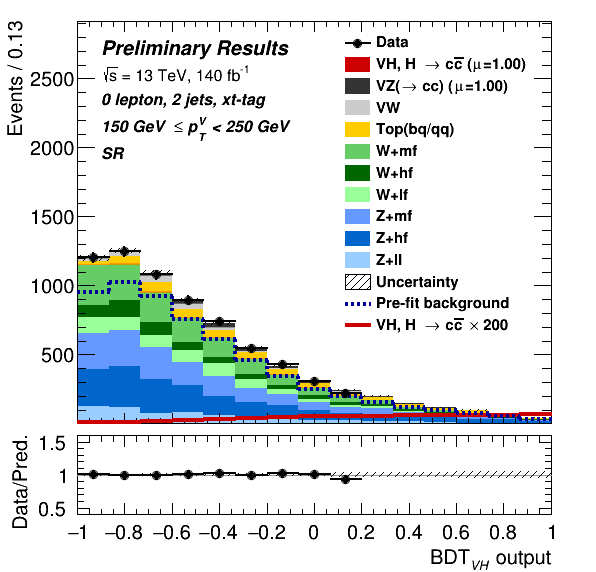
\includegraphics[width=0.32\textwidth]{Images/VH/Own_fit/postfit_VHcc/Region_distmva_BMax250_BMin150_DSR_J2_TTypext_T2_L0_Y6051_GlobalFit_conditionnal_mu1.png}
        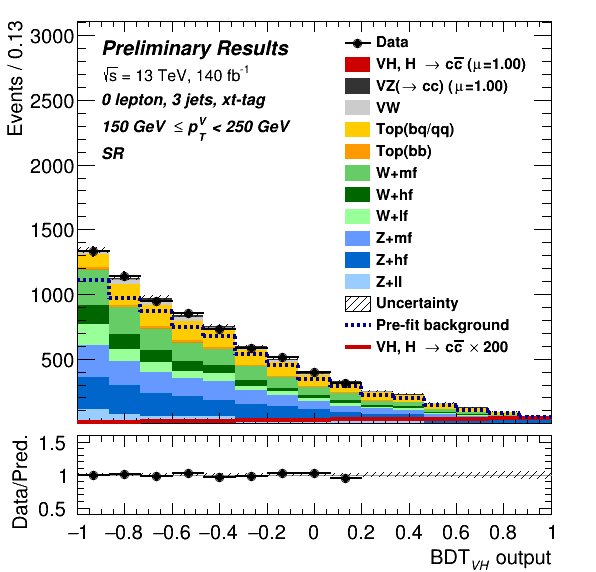
\includegraphics[width=0.32\textwidth]{Images/VH/Own_fit/postfit_VHcc/Region_distmva_BMax250_BMin150_DSR_J3_TTypext_T2_L0_Y6051_GlobalFit_conditionnal_mu1.png}
        \caption{150 < \ptv\ < 250 GeV.}
        \label{fig:plots_VHcc_OL_150_SR_2c}
    \end{subfigure}
    \begin{subfigure}[b]{\textwidth}
        \centering
        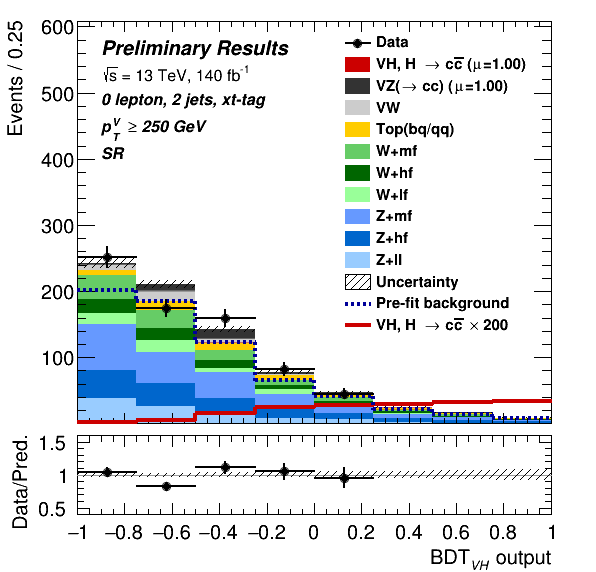
\includegraphics[width=0.32\textwidth]{Images/VH/Own_fit/postfit_VHcc/Region_distmva_BMin250_DSR_J2_TTypext_T2_L0_Y6051_GlobalFit_conditionnal_mu1.png}
        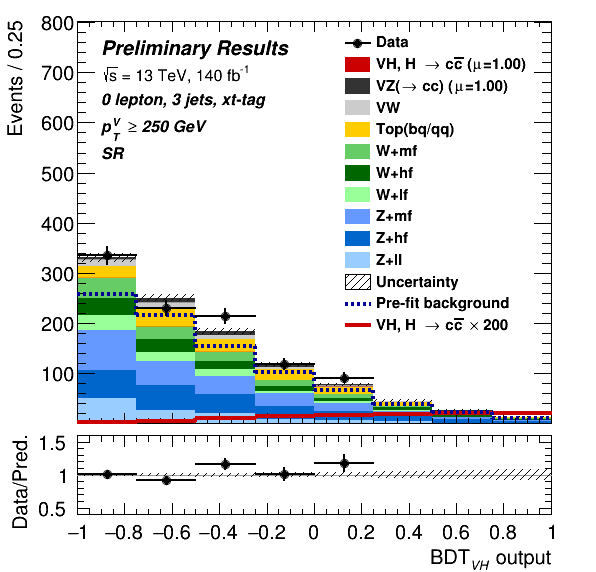
\includegraphics[width=0.32\textwidth]{Images/VH/Own_fit/postfit_VHcc/Region_distmva_BMin250_DSR_J3_TTypext_T2_L0_Y6051_GlobalFit_conditionnal_mu1.png}
        \caption{250 GeV < \ptv.}
        \label{fig:plots_VHcc_OL_250_SR_2c}
    \end{subfigure}
    \caption{\gls{bdt} distributions in the 0L 2 $c$-tagged signal regions, 2-jet (left) and 3-jet (right).}
    \label{fig:plots_VHcc_OL_SR_2c}
\end{figure} 
\begin{figure}[h!]
    \centering
    \begin{subfigure}[b]{\textwidth}
        \centering
        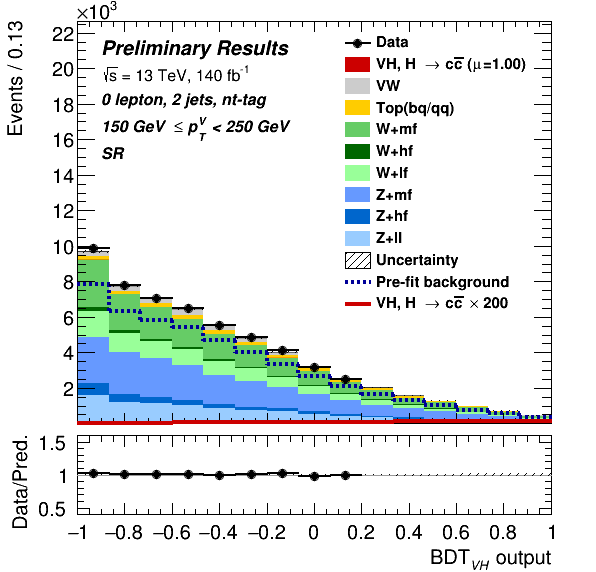
\includegraphics[width=0.32\textwidth]{Images/VH/Own_fit/postfit_VHcc/Region_distmva_BMax250_BMin150_DSR_J2_TTypent_T1_L0_Y6051_GlobalFit_conditionnal_mu1.png}
        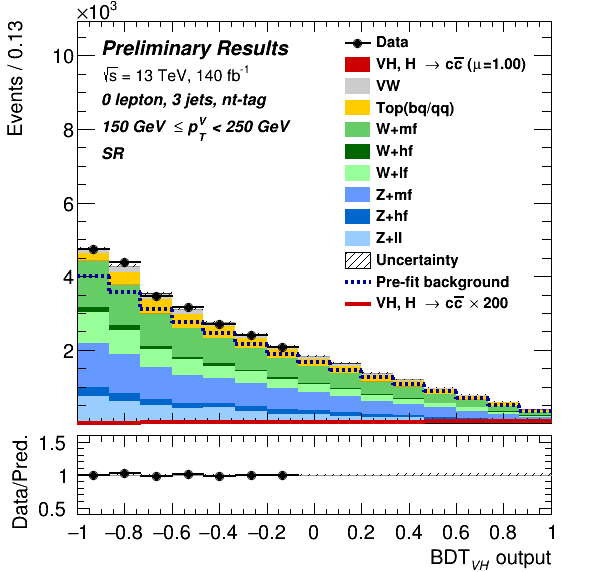
\includegraphics[width=0.32\textwidth]{Images/VH/Own_fit/postfit_VHcc/Region_distmva_BMax250_BMin150_DSR_J3_TTypent_T1_L0_Y6051_GlobalFit_conditionnal_mu1.png}
        \caption{150 < \ptv\ < 250 GeV.}
        \label{fig:plots_VHcc_OL_150_SR_1c}
    \end{subfigure}
    \begin{subfigure}[b]{\textwidth}
        \centering
        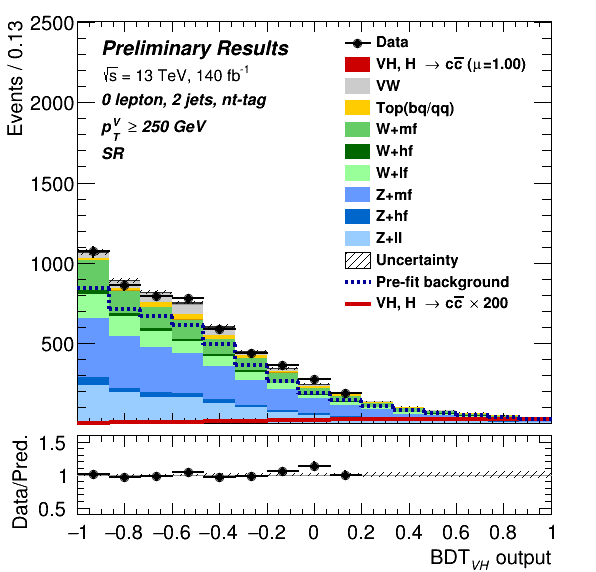
\includegraphics[width=0.32\textwidth]{Images/VH/Own_fit/postfit_VHcc/Region_distmva_BMin250_DSR_J2_TTypent_T1_L0_Y6051_GlobalFit_conditionnal_mu1.png}
        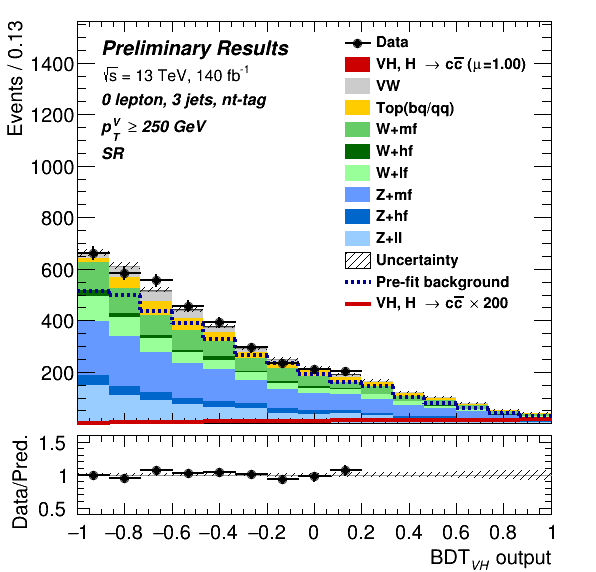
\includegraphics[width=0.32\textwidth]{Images/VH/Own_fit/postfit_VHcc/Region_distmva_BMin250_DSR_J3_TTypent_T1_L0_Y6051_GlobalFit_conditionnal_mu1.png}
        \caption{250 GeV < \ptv.}
        \label{fig:plots_VHcc_OL_250_SR_1c}
    \end{subfigure}
    \caption{\gls{bdt} distributions in the 0L 1 $c$-tagged signal regions, 2-jet (left) and 3-jet (right).}
    \label{fig:plots_VHcc_OL_SR_1c}
\end{figure} 

\vspace*{\fill} 

\begin{figure}[h!]
    \centering
    \begin{subfigure}[b]{\textwidth}
        \centering
        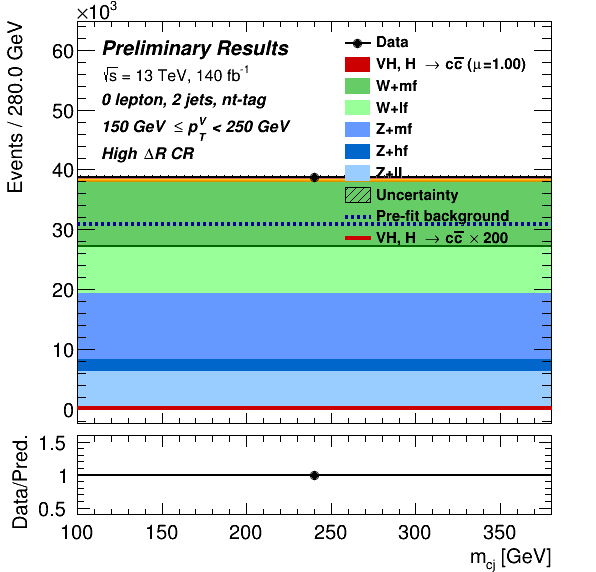
\includegraphics[width=0.32\textwidth]{Images/VH/Own_fit/postfit_VHcc/Region_distmBB_BMax250_BMin150_DCRHigh_J2_TTypent_T1_L0_Y6051_GlobalFit_conditionnal_mu1.png}
        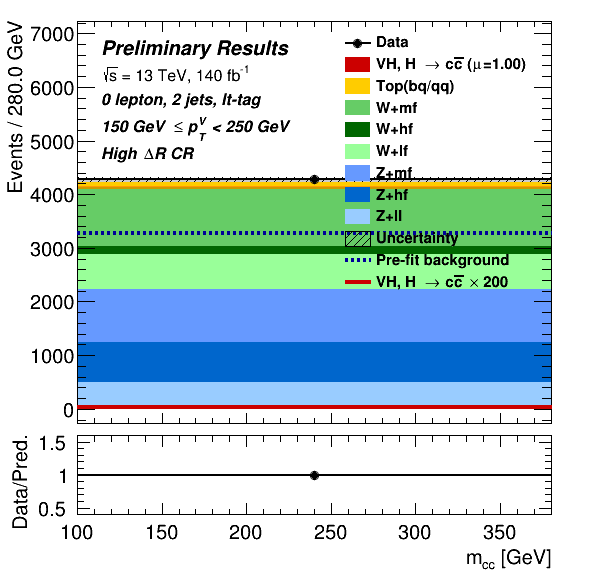
\includegraphics[width=0.32\textwidth]{Images/VH/Own_fit/postfit_VHcc/Region_distmBB_BMax250_BMin150_DCRHigh_J2_TTypelt_T2_L0_Y6051_GlobalFit_conditionnal_mu1.png}
        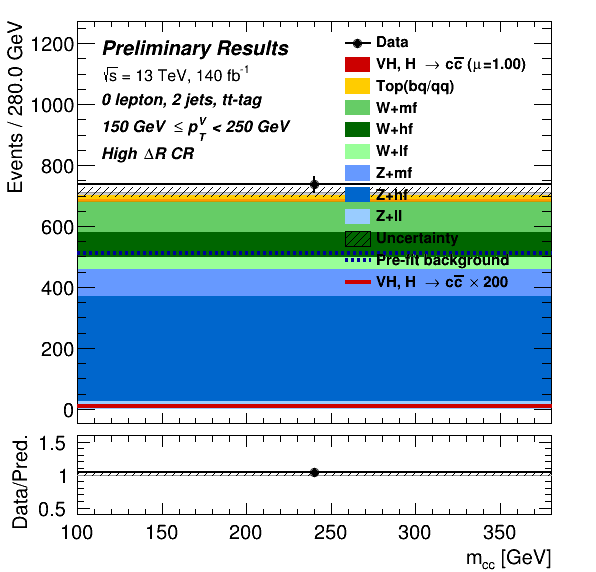
\includegraphics[width=0.32\textwidth]{Images/VH/Own_fit/postfit_VHcc/Region_distmBB_BMax250_BMin150_DCRHigh_J2_TTypett_T2_L0_Y6051_GlobalFit_conditionnal_mu1.png}
        \caption{150 < \ptv\ < 250 GeV, $TN$- (left), $LT$- (centre), and $TT$-tag (right).}
        \label{fig:plots_VHcc_OL_150_CRH_2c_2J}
    \end{subfigure}
    \begin{subfigure}[b]{\textwidth}
        \centering
        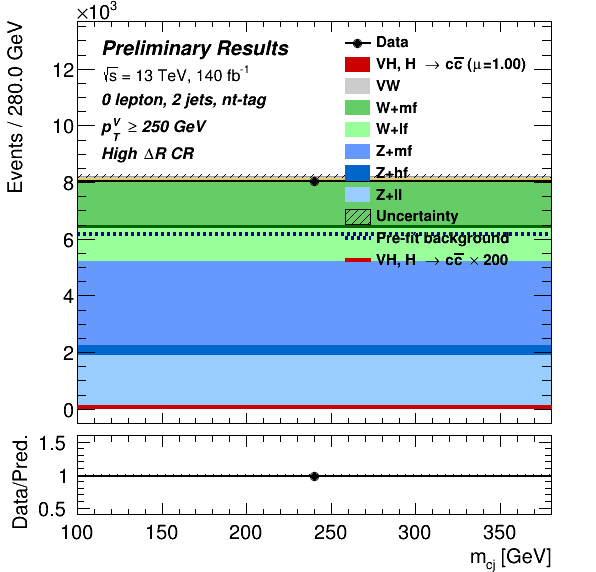
\includegraphics[width=0.32\textwidth]{Images/VH/Own_fit/postfit_VHcc/Region_distmBB_BMin250_DCRHigh_J2_TTypent_T1_L0_Y6051_GlobalFit_conditionnal_mu1.png}
        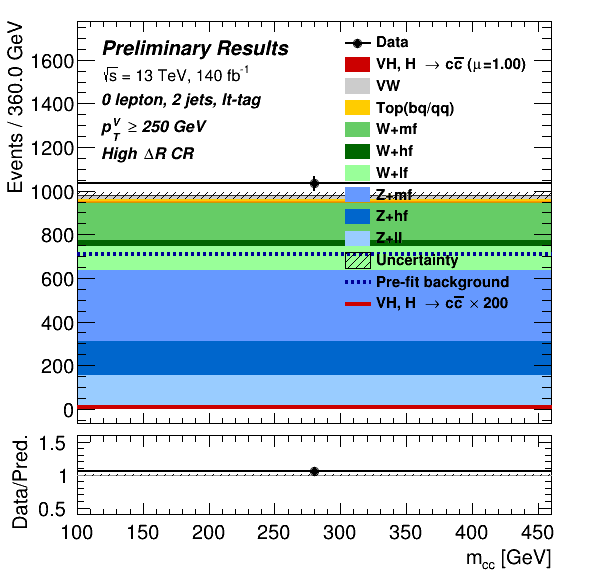
\includegraphics[width=0.32\textwidth]{Images/VH/Own_fit/postfit_VHcc/Region_distmBB_BMin250_DCRHigh_J2_TTypelt_T2_L0_Y6051_GlobalFit_conditionnal_mu1.png}
        \includegraphics[width=0.32\textwidth]{Images/VH/Own_fit/postfit_VHcc/Region_distmBB_BMin250_DCRHigh_J2_TTypett_T2_L0_Y6051_GlobalFit_conditionnal_mu1.png}
        \caption{250 GeV < \ptv, $TN$- (left), $LT$- (centre), and $TT$-tag (right).}
        \label{fig:plots_VHcc_OL_250_CRH_2c_2J}
    \end{subfigure}
    \caption{$H$-candidate mass distributions in the 0L 2-jet \highdr\ CRs.}
    \label{fig:plots_VHcc_OL_CRH_2c_2J}
\end{figure} 
\begin{figure}[h!]
    \centering
    \begin{subfigure}[b]{\textwidth}
        \centering
        \includegraphics[width=0.32\textwidth]{Images/VH/Own_fit/postfit_VHcc/Region_distmBB_BMax250_BMin150_DCRHigh_J3_TTypent_T1_L0_Y6051_GlobalFit_conditionnal_mu1.png}
        \includegraphics[width=0.32\textwidth]{Images/VH/Own_fit/postfit_VHcc/Region_distmBB_BMax250_BMin150_DCRHigh_J3_TTypelt_T2_L0_Y6051_GlobalFit_conditionnal_mu1.png}
        \includegraphics[width=0.32\textwidth]{Images/VH/Own_fit/postfit_VHcc/Region_distmBB_BMax250_BMin150_DCRHigh_J3_TTypett_T2_L0_Y6051_GlobalFit_conditionnal_mu1.png}
        \caption{150 GeV < \ptv\ < 250 GeV, $TN$- (left), $LT$- (centre), and $TT$-tag (right).}
        \label{fig:plots_VHcc_OL_150_CRH_2c_3J}
    \end{subfigure}
    \begin{subfigure}[b]{\textwidth}
        \centering

        \includegraphics[width=0.32\textwidth]{Images/VH/Own_fit/postfit_VHcc/Region_distmBB_BMin250_DCRHigh_J3_TTypent_T1_L0_Y6051_GlobalFit_conditionnal_mu1.png}
        \includegraphics[width=0.32\textwidth]{Images/VH/Own_fit/postfit_VHcc/Region_distmBB_BMin250_DCRHigh_J3_TTypelt_T2_L0_Y6051_GlobalFit_conditionnal_mu1.png}
        \includegraphics[width=0.32\textwidth]{Images/VH/Own_fit/postfit_VHcc/Region_distmBB_BMin250_DCRHigh_J3_TTypett_T2_L0_Y6051_GlobalFit_conditionnal_mu1.png}
        \caption{250 GeV < \ptv, $TN$- (left), $LT$- (centre), and $TT$-tag (right).}
        \label{fig:plots_VHcc_OL_250_CRH_2c_3J}
    \end{subfigure}
    \caption{$H$-candidate mass distributions in the 0L 3-jet \highdr\ CRs.}
    \label{fig:plots_VHcc_OL_CRH_2c_3J}
\end{figure} 

\vspace*{\fill} 

% TopCR 0L
\begin{figure}[h!]
    \centering
    \begin{subfigure}[b]{\textwidth}
        \centering
        \includegraphics[width=0.32\textwidth]{Images/VH/Own_fit/postfit_VHcc/Region_distmBB_BMax250_BMin150_DtopCRBC_J2_TTypebt_T1_L0_Y6051_GlobalFit_conditionnal_mu1.png}
        \includegraphics[width=0.32\textwidth]{Images/VH/Own_fit/postfit_VHcc/Region_distmBB_BMax250_BMin150_DtopCRBC_J3_TTypebt_T1_L0_Y6051_GlobalFit_conditionnal_mu1.png}
        \includegraphics[width=0.32\textwidth]{Images/VH/Own_fit/postfit_VHbb/Region_distmBB_BMax250_BMin150_DtopCRBC_J4_TTypebt_T1_L0_Y6051_GlobalFit_conditionnal_mu1.png} % Must be VHbb due to 4j
        \caption{150 < \ptv\ < 250 GeV.}
        \label{fig:plots_VHcc_OL_150_TopCR_2c}
    \end{subfigure}
    \begin{subfigure}[b]{\textwidth}
        \centering
        \includegraphics[width=0.32\textwidth]{Images/VH/Own_fit/postfit_VHcc/Region_distmBB_BMax400_BMin250_DtopCRBC_J2_TTypebt_T1_L0_Y6051_GlobalFit_conditionnal_mu1.png}
        \includegraphics[width=0.32\textwidth]{Images/VH/Own_fit/postfit_VHcc/Region_distmBB_BMax400_BMin250_DtopCRBC_J3_TTypebt_T1_L0_Y6051_GlobalFit_conditionnal_mu1.png}
        \includegraphics[width=0.32\textwidth]{Images/VH/Own_fit/postfit_VHbb/Region_distmBB_BMax400_BMin250_DtopCRBC_J4_TTypebt_T1_L0_Y6051_GlobalFit_conditionnal_mu1.png} % Must be VHbb due to 4j
        \caption{250 GeV < \ptv\ < 400 GeV.}
        \label{fig:plots_VHcc_OL_250_TopCR_2c}
    \end{subfigure}
    \caption{$H$-candidate mass distributions in the 0L $BT$-tagged Top CRs, 2-jet (left), 3-jet (centre), and 4-jet (right).}
    \label{fig:plots_VHcc_OL_TopCR_2c}
\end{figure} 

\vspace*{\fill} \newpage
\vspace*{\fill} 

% 1L
\begin{figure}[h!]
    \centering
    \begin{subfigure}[b]{\textwidth}
        \centering
        \includegraphics[width=0.32\textwidth]{Images/VH/Own_fit/postfit_VHcc/Region_distmva_BMax150_BMin75_DSR_J2_TTypext_T2_L1_Y6051_GlobalFit_conditionnal_mu1.png}
        \includegraphics[width=0.32\textwidth]{Images/VH/Own_fit/postfit_VHcc/Region_distmva_BMax250_BMin150_DSR_J2_TTypext_T2_L1_Y6051_GlobalFit_conditionnal_mu1.png}
        \includegraphics[width=0.32\textwidth]{Images/VH/Own_fit/postfit_VHcc/Region_distmva_BMin250_DSR_J2_TTypext_T2_L1_Y6051_GlobalFit_conditionnal_mu1.png}
        \caption{2-jet, [75, 150] GeV (left), [150, 250] GeV (centre), and 250  GeV $\leq$ (right) \ptv\ regions.}
        \label{fig:plots_VHcc_1L_SR_2J_2c}
    \end{subfigure}
    \begin{subfigure}[b]{\textwidth}
        \centering
        \includegraphics[width=0.32\textwidth]{Images/VH/Own_fit/postfit_VHcc/Region_distmva_BMax150_BMin75_DSR_J3_TTypext_T2_L1_Y6051_GlobalFit_conditionnal_mu1.png}
        \includegraphics[width=0.32\textwidth]{Images/VH/Own_fit/postfit_VHcc/Region_distmva_BMax250_BMin150_DSR_J3_TTypext_T2_L1_Y6051_GlobalFit_conditionnal_mu1.png}
        \includegraphics[width=0.32\textwidth]{Images/VH/Own_fit/postfit_VHcc/Region_distmva_BMin250_DSR_J3_TTypext_T2_L1_Y6051_GlobalFit_conditionnal_mu1.png}
        \caption{3-jet, [75, 150] GeV (left), [150, 250] GeV (centre), and 250  GeV $\leq$ (right) \ptv\ regions.}
        \label{fig:plots_VHcc_1L_SR_3J_2c}
    \end{subfigure}
    \caption{\gls{bdt} distributions in the 1L 2 $c$-tagged signal regions.}
    \label{fig:plots_VHcc_1L_SR_2c}
\end{figure}
\begin{figure}[h!]
    \centering
    \begin{subfigure}[b]{\textwidth}
        \centering
        \includegraphics[width=0.32\textwidth]{Images/VH/Own_fit/postfit_VHcc/Region_distmva_BMax250_BMin150_DSR_J2_TTypent_T1_L1_Y6051_GlobalFit_conditionnal_mu1.png}
        \includegraphics[width=0.32\textwidth]{Images/VH/Own_fit/postfit_VHcc/Region_distmva_BMin250_DSR_J2_TTypent_T1_L1_Y6051_GlobalFit_conditionnal_mu1.png}
        \caption{2-jet, [75, 150] GeV (left), [150, 250] GeV (centre), and 250  GeV $\leq$ (right) \ptv\ regions.}
        \label{fig:plots_VHcc_1L_SR_2J_1c}
    \end{subfigure}
    \begin{subfigure}[b]{\textwidth}
        \centering
        \includegraphics[width=0.32\textwidth]{Images/VH/Own_fit/postfit_VHcc/Region_distmva_BMax250_BMin150_DSR_J3_TTypent_T1_L1_Y6051_GlobalFit_conditionnal_mu1.png}
        \includegraphics[width=0.32\textwidth]{Images/VH/Own_fit/postfit_VHcc/Region_distmva_BMin250_DSR_J3_TTypent_T1_L1_Y6051_GlobalFit_conditionnal_mu1.png}
        \caption{3-jet, [75, 150] GeV (left), [150, 250] GeV (centre), and 250  GeV $\leq$ (right) \ptv\ regions.}
        \label{fig:plots_VHcc_1L_SR_3J_1c}
    \end{subfigure}
    \caption{\gls{bdt} distributions in the 1L 1 $c$-tagged signal regions.}
    \label{fig:plots_VHcc_1L_SR_1c}
\end{figure}

\newpage
\vspace*{\fill} 


\begin{figure}[h!]
    \centering
    \begin{subfigure}[b]{\textwidth}
        \centering
        \includegraphics[width=0.32\textwidth]{Images/VH/Own_fit/blank.png}
        \includegraphics[width=0.32\textwidth]{Images/VH/Own_fit/postfit_VHcc/Region_distmBB_BMax150_BMin75_DCRHigh_J2_TTypelt_T2_L1_Y6051_GlobalFit_conditionnal_mu1.png}
        \includegraphics[width=0.32\textwidth]{Images/VH/Own_fit/postfit_VHcc/Region_distmBB_BMax150_BMin75_DCRHigh_J2_TTypett_T2_L1_Y6051_GlobalFit_conditionnal_mu1.png}
        \caption{75 < \ptv\ < 150 GeV ($TN$ not included).}
        \label{fig:plots_VHcc_1L_75_CRH_2J}
    \end{subfigure}
    \begin{subfigure}[b]{\textwidth}
        \centering
        \includegraphics[width=0.32\textwidth]{Images/VH/Own_fit/postfit_VHcc/Region_distpTV_BMax250_BMin150_DCRHigh_J2_TTypent_T1_L1_Y6051_GlobalFit_conditionnal_mu1.png}
        \includegraphics[width=0.32\textwidth]{Images/VH/Own_fit/postfit_VHcc/Region_distmBB_BMax250_BMin150_DCRHigh_J2_TTypelt_T2_L1_Y6051_GlobalFit_conditionnal_mu1.png}
        \includegraphics[width=0.32\textwidth]{Images/VH/Own_fit/postfit_VHcc/Region_distmBB_BMax250_BMin150_DCRHigh_J2_TTypett_T2_L1_Y6051_GlobalFit_conditionnal_mu1.png}
        \caption{150 < \ptv\ < 250 GeV.}
        \label{fig:plots_VHcc_1L_150_CRH_2J}
    \end{subfigure}
    \begin{subfigure}[b]{\textwidth}
        \centering
        \includegraphics[width=0.32\textwidth]{Images/VH/Own_fit/postfit_VHcc/Region_distpTV_BMin250_DCRHigh_J2_TTypent_T1_L1_Y6051_GlobalFit_conditionnal_mu1.png}
        \includegraphics[width=0.32\textwidth]{Images/VH/Own_fit/postfit_VHcc/Region_distmBB_BMin250_DCRHigh_J2_TTypelt_T2_L1_Y6051_GlobalFit_conditionnal_mu1.png}
        \includegraphics[width=0.32\textwidth]{Images/VH/Own_fit/postfit_VHcc/Region_distmBB_BMin250_DCRHigh_J2_TTypett_T2_L1_Y6051_GlobalFit_conditionnal_mu1.png}
        \caption{250 GeV < \ptv.}
        \label{fig:plots_VHcc_1L_250_CRH_2J}
    \end{subfigure}
    \caption{$TN$-tagged \ptv\ distributions (left) and $LT$- (centre) and $TT$-tagged (right) $H$-candidate mass distributions in the 1L \highdr\ CR 2-jet regions.}
    \label{fig:plots_VHcc_1L_CRH_2J}
\end{figure}

\vspace*{\fill} \newpage
\vspace*{\fill} 

\begin{figure}[h!]
    \centering
    \begin{subfigure}[b]{\textwidth}
        \centering
        \includegraphics[width=0.32\textwidth]{Images/VH/Own_fit/blank.png}
        \includegraphics[width=0.32\textwidth]{Images/VH/Own_fit/postfit_VHcc/Region_distmBB_BMax150_BMin75_DCRHigh_J3_TTypelt_T2_L1_Y6051_GlobalFit_conditionnal_mu1.png}
        \includegraphics[width=0.32\textwidth]{Images/VH/Own_fit/postfit_VHcc/Region_distmBB_BMax150_BMin75_DCRHigh_J3_TTypett_T2_L1_Y6051_GlobalFit_conditionnal_mu1.png}
        \caption{75 < \ptv\ < 150 GeV ($TN$ not included).}
        \label{fig:plots_VHcc_1L_75_CRH_3J}
    \end{subfigure}
    \begin{subfigure}[b]{\textwidth}
        \centering
        \includegraphics[width=0.32\textwidth]{Images/VH/Own_fit/postfit_VHcc/Region_distpTV_BMax250_BMin150_DCRHigh_J3_TTypent_T1_L1_Y6051_GlobalFit_conditionnal_mu1.png}
        \includegraphics[width=0.32\textwidth]{Images/VH/Own_fit/postfit_VHcc/Region_distmBB_BMax250_BMin150_DCRHigh_J3_TTypelt_T2_L1_Y6051_GlobalFit_conditionnal_mu1.png}
        \includegraphics[width=0.32\textwidth]{Images/VH/Own_fit/postfit_VHcc/Region_distmBB_BMax250_BMin150_DCRHigh_J3_TTypett_T2_L1_Y6051_GlobalFit_conditionnal_mu1.png}
        \caption{150 < \ptv\ < 250 GeV.}
        \label{fig:plots_VHcc_1L_150_CRH_3J}
    \end{subfigure}
    \begin{subfigure}[b]{\textwidth}
        \centering
        \includegraphics[width=0.32\textwidth]{Images/VH/Own_fit/postfit_VHcc/Region_distpTV_BMin250_DCRHigh_J3_TTypent_T1_L1_Y6051_GlobalFit_conditionnal_mu1.png}
        \includegraphics[width=0.32\textwidth]{Images/VH/Own_fit/postfit_VHcc/Region_distmBB_BMin250_DCRHigh_J3_TTypelt_T2_L1_Y6051_GlobalFit_conditionnal_mu1.png}
        \includegraphics[width=0.32\textwidth]{Images/VH/Own_fit/postfit_VHcc/Region_distmBB_BMin250_DCRHigh_J3_TTypett_T2_L1_Y6051_GlobalFit_conditionnal_mu1.png}
        \caption{250 GeV < \ptv.}
        \label{fig:plots_VHcc_1L_250_CRH_3J}
    \end{subfigure}
    \caption{$TN$-tagged \ptv\ distributions (left) and $LT$- (centre) and $TT$-tagged (right) $H$-candidate mass distributions in the 1L \highdr\ CR 3-jet regions.}
    \label{fig:plots_VHcc_1L_CRH_3J}
\end{figure}

\vspace*{\fill} \newpage

\begin{figure}[h!]
    \centering
    \begin{subfigure}[b]{\textwidth}
        \centering
        \includegraphics[width=0.32\textwidth]{Images/VH/Own_fit/postfit_VHcc/Region_distmBB_BMax150_BMin75_DtopCRBC_J2_TTypebt_T1_L1_Y6051_GlobalFit_conditionnal_mu1.png}
        \includegraphics[width=0.32\textwidth]{Images/VH/Own_fit/postfit_VHcc/Region_distmBB_BMax250_BMin150_DtopCRBC_J2_TTypebt_T1_L1_Y6051_GlobalFit_conditionnal_mu1.png}
        \includegraphics[width=0.32\textwidth]{Images/VH/Own_fit/postfit_VHcc/Region_distmBB_BMax400_BMin250_DtopCRBC_J2_TTypebt_T1_L1_Y6051_GlobalFit_conditionnal_mu1.png}
        \caption{2-jet, [75, 150] GeV (left), [150, 250] GeV (centre), and 250 GeV $\leq$ (right) \ptv\ regions.}
        \label{fig:plots_VHcc_1L_TopCR_2J}
    \end{subfigure}
    \begin{subfigure}[b]{\textwidth}
        \centering
        \includegraphics[width=0.32\textwidth]{Images/VH/Own_fit/postfit_VHcc/Region_distmBB_BMax150_BMin75_DtopCRBC_J3_TTypebt_T1_L1_Y6051_GlobalFit_conditionnal_mu1.png}
        \includegraphics[width=0.32\textwidth]{Images/VH/Own_fit/postfit_VHcc/Region_distmBB_BMax250_BMin150_DtopCRBC_J3_TTypebt_T1_L1_Y6051_GlobalFit_conditionnal_mu1.png}
        \includegraphics[width=0.32\textwidth]{Images/VH/Own_fit/postfit_VHcc/Region_distmBB_BMax400_BMin250_DtopCRBC_J3_TTypebt_T1_L1_Y6051_GlobalFit_conditionnal_mu1.png}
        \caption{3-jet, [75, 150] GeV (left), [150, 250] GeV (centre), and 250 GeV $\leq$ (right) \ptv\ regions.}
        \label{fig:plots_VHcc_1L_TopCR_3J}
    \end{subfigure}
    \caption{$H$-candidate mass distribution in the 1L $BT$-tagged Top CRs.}
    \label{fig:plots_VHcc_1L_TopCR}
\end{figure}
\begin{figure}[h!]
    \centering
    \begin{subfigure}[b]{\textwidth}
        \centering
        \includegraphics[width=0.32\textwidth]{Images/VH/Own_fit/postfit_VHcc/Region_distpTV_BMax250_BMin150_DSR_J2_TTypeln_T1_L1_Y6051_GlobalFit_conditionnal_mu1.png}
        \includegraphics[width=0.32\textwidth]{Images/VH/Own_fit/postfit_VHcc/Region_distpTV_BMin250_DSR_J2_TTypeln_T1_L1_Y6051_GlobalFit_conditionnal_mu1.png}
        \caption{2-jet.}
        \label{fig:plots_VHcc_1L_LN_2J}
    \end{subfigure}
    \begin{subfigure}[b]{\textwidth}
        \centering
        \includegraphics[width=0.32\textwidth]{Images/VH/Own_fit/postfit_VHcc/Region_distpTV_BMax250_BMin150_DSR_J3_TTypeln_T1_L1_Y6051_GlobalFit_conditionnal_mu1.png}
        \includegraphics[width=0.32\textwidth]{Images/VH/Own_fit/postfit_VHcc/Region_distpTV_BMin250_DSR_J3_TTypeln_T1_L1_Y6051_GlobalFit_conditionnal_mu1.png}
        \caption{3-jet.}
        \label{fig:plots_VHcc_1L_SR_3J}
    \end{subfigure}
    \caption{\ptv\ distributions in the 1L $LN$-tagged $V+l$ CR [150, 250] GeV (left) and 250 GeV $\leq$ (right) \ptv\ regions.}
    \label{fig:plots_VHcc_1L_LN}
\end{figure}

\newpage

% 2L
\vspace*{\fill} 

\begin{figure}[h!]
    \centering
    \begin{subfigure}[b]{\textwidth}
        \centering
        \includegraphics[width=0.32\textwidth]{Images/VH/Own_fit/postfit_VHcc/Region_distmva_BMax150_BMin75_DSR_J2_TTypext_T2_L2_Y6051_GlobalFit_conditionnal_mu1.png}
        \includegraphics[width=0.32\textwidth]{Images/VH/Own_fit/postfit_VHcc/Region_distmva_BMax250_BMin150_DSR_J2_TTypext_T2_L2_Y6051_GlobalFit_conditionnal_mu1.png}
        \includegraphics[width=0.32\textwidth]{Images/VH/Own_fit/postfit_VHcc/Region_distmva_BMin250_DSR_J2_TTypext_T2_L2_Y6051_GlobalFit_conditionnal_mu1.png}
        \caption{2-jet, [75, 150] GeV (left), [150, 250] GeV (centre), and 250  GeV $\leq$ (right) \ptv\ regions.}
        \label{fig:plots_VHcc_2L_SR_2c_2J}
    \end{subfigure}
    \begin{subfigure}[b]{\textwidth}
        \centering
        \includegraphics[width=0.32\textwidth]{Images/VH/Own_fit/postfit_VHcc/Region_distmva_BMax150_BMin75_DSR_J3_TTypext_incJet1_T2_L2_Y6051_GlobalFit_conditionnal_mu1.png}
        \includegraphics[width=0.32\textwidth]{Images/VH/Own_fit/postfit_VHcc/Region_distmva_BMax250_BMin150_DSR_J3_TTypext_incJet1_T2_L2_Y6051_GlobalFit_conditionnal_mu1.png}
        \includegraphics[width=0.32\textwidth]{Images/VH/Own_fit/postfit_VHcc/Region_distmva_BMin250_DSR_J3_TTypext_incJet1_T2_L2_Y6051_GlobalFit_conditionnal_mu1.png}
        \caption{$\geq$3-jet, [75, 150] GeV (left), [150, 250] GeV (centre), and 250  GeV $\leq$ (right) \ptv\ regions.}
        \label{fig:plots_VHcc_2L_SR_2c_3J}
    \end{subfigure}
    \caption{\gls{bdt} distributions in the 2L 2 $c$-tagged signal regions.}
    \label{fig:plots_VHcc_2L_SR_2c}
\end{figure}
\begin{figure}[h!]
    \centering
    \begin{subfigure}[b]{\textwidth}
        \centering
        \includegraphics[width=0.32\textwidth]{Images/VH/Own_fit/postfit_VHcc/Region_distmva_BMax150_BMin75_DSR_J2_TTypent_T1_L2_Y6051_GlobalFit_conditionnal_mu1.png}
        \includegraphics[width=0.32\textwidth]{Images/VH/Own_fit/postfit_VHcc/Region_distmva_BMax250_BMin150_DSR_J2_TTypent_T1_L2_Y6051_GlobalFit_conditionnal_mu1.png}
        \includegraphics[width=0.32\textwidth]{Images/VH/Own_fit/postfit_VHcc/Region_distmva_BMin250_DSR_J2_TTypent_T1_L2_Y6051_GlobalFit_conditionnal_mu1.png}
        \caption{2-jet, [75, 150] GeV (left), [150, 250] GeV (centre), and 250  GeV $\leq$ (right) \ptv\ regions.}
        \label{fig:plots_VHcc_2L_SR_1c_2J}
    \end{subfigure}
    \begin{subfigure}[b]{\textwidth}
        \centering
        \includegraphics[width=0.32\textwidth]{Images/VH/Own_fit/postfit_VHcc/Region_distmva_BMax150_BMin75_DSR_J3_TTypent_incJet1_T1_L2_Y6051_GlobalFit_conditionnal_mu1.png}
        \includegraphics[width=0.32\textwidth]{Images/VH/Own_fit/postfit_VHcc/Region_distmva_BMax250_BMin150_DSR_J3_TTypent_incJet1_T1_L2_Y6051_GlobalFit_conditionnal_mu1.png}
        \includegraphics[width=0.32\textwidth]{Images/VH/Own_fit/postfit_VHcc/Region_distmva_BMin250_DSR_J3_TTypent_incJet1_T1_L2_Y6051_GlobalFit_conditionnal_mu1.png}
        \caption{$\geq$3-jet, [75, 150] GeV (left), [150, 250] GeV (centre), and 250  GeV $\leq$ (right) \ptv\ regions.}
        \label{fig:plots_VHcc_2L_SR_1c_3J}
    \end{subfigure}
    \caption{\gls{bdt} distributions in the 2L 1 $c$-tagged signal regions.}
    \label{fig:plots_VHcc_2L_SR_1c}
\end{figure}

\newpage
\vspace*{\fill} 


\begin{figure}[h!]
    \centering
    \begin{subfigure}[b]{\textwidth}
        \centering
        \includegraphics[width=0.32\textwidth]{Images/VH/Own_fit/postfit_VHcc/Region_distpTV_BMax150_BMin75_DCRHigh_J2_TTypent_T1_L2_Y6051_GlobalFit_conditionnal_mu1.png}
        \includegraphics[width=0.32\textwidth]{Images/VH/Own_fit/postfit_VHcc/Region_distmBB_BMax150_BMin75_DCRHigh_J2_TTypelt_T2_L2_Y6051_GlobalFit_conditionnal_mu1.png}
        \includegraphics[width=0.32\textwidth]{Images/VH/Own_fit/postfit_VHcc/Region_distmBB_BMax150_BMin75_DCRHigh_J2_TTypett_T2_L2_Y6051_GlobalFit_conditionnal_mu1.png}
        \caption{75 < \ptv\ < 150 GeV.}
        \label{fig:plots_VHcc_2L_75_CRH_2J}
    \end{subfigure}
    \begin{subfigure}[b]{\textwidth}
        \centering
        \includegraphics[width=0.32\textwidth]{Images/VH/Own_fit/postfit_VHcc/Region_distpTV_BMax250_BMin150_DCRHigh_J2_TTypent_T1_L2_Y6051_GlobalFit_conditionnal_mu1.png}
        \includegraphics[width=0.32\textwidth]{Images/VH/Own_fit/postfit_VHcc/Region_distmBB_BMax250_BMin150_DCRHigh_J2_TTypelt_T2_L2_Y6051_GlobalFit_conditionnal_mu1.png}
        \includegraphics[width=0.32\textwidth]{Images/VH/Own_fit/postfit_VHcc/Region_distmBB_BMax250_BMin150_DCRHigh_J2_TTypett_T2_L2_Y6051_GlobalFit_conditionnal_mu1.png}
        \caption{150 < \ptv\ < 250 GeV.}
        \label{fig:plots_VHcc_2L_150_CRH_2J}
    \end{subfigure}
    \begin{subfigure}[b]{\textwidth}
        \centering
        \includegraphics[width=0.32\textwidth]{Images/VH/Own_fit/postfit_VHcc/Region_distpTV_BMin250_DCRHigh_J2_TTypent_T1_L2_Y6051_GlobalFit_conditionnal_mu1.png}
        \includegraphics[width=0.32\textwidth]{Images/VH/Own_fit/postfit_VHcc/Region_distmBB_BMin250_DCRHigh_J2_TTypelt_T2_L2_Y6051_GlobalFit_conditionnal_mu1.png}
        \includegraphics[width=0.32\textwidth]{Images/VH/Own_fit/postfit_VHcc/Region_distmBB_BMin250_DCRHigh_J2_TTypett_T2_L2_Y6051_GlobalFit_conditionnal_mu1.png}
        \caption{250 GeV < \ptv.}
        \label{fig:plots_VHcc_2L_250_CRH_2J}
    \end{subfigure}
    \caption{$TN$-tagged \ptv\ distributions (left) and the $LT$- (centre) and $TT$-tagged (right) $H$-candidate mass distributions in the 2L \highdr\ CR 2-jet regions.}
    \label{fig:plots_VHcc_2L_CRH_3J}
\end{figure}

\vspace*{\fill} \newpage
\vspace*{\fill} 

\begin{figure}[h!]
    \centering
    \begin{subfigure}[b]{\textwidth}
        \centering
        \includegraphics[width=0.32\textwidth]{Images/VH/Own_fit/postfit_VHcc/Region_distpTV_BMax150_BMin75_DCRHigh_J3_TTypent_incJet1_T1_L2_Y6051_GlobalFit_conditionnal_mu1.png}
        \includegraphics[width=0.32\textwidth]{Images/VH/Own_fit/postfit_VHcc/Region_distmBB_BMax150_BMin75_DCRHigh_J3_TTypelt_incJet1_T2_L2_Y6051_GlobalFit_conditionnal_mu1.png}
        \includegraphics[width=0.32\textwidth]{Images/VH/Own_fit/postfit_VHcc/Region_distmBB_BMax150_BMin75_DCRHigh_J3_TTypett_incJet1_T2_L2_Y6051_GlobalFit_conditionnal_mu1.png}
        \caption{75 < \ptv\ < 150 GeV.}
        \label{fig:plots_VHcc_2L_75_CRH_3J}
    \end{subfigure}
    \begin{subfigure}[b]{\textwidth}
        \centering
        \includegraphics[width=0.32\textwidth]{Images/VH/Own_fit/postfit_VHcc/Region_distpTV_BMax250_BMin150_DCRHigh_J3_TTypent_incJet1_T1_L2_Y6051_GlobalFit_conditionnal_mu1.png}
        \includegraphics[width=0.32\textwidth]{Images/VH/Own_fit/postfit_VHcc/Region_distmBB_BMax250_BMin150_DCRHigh_J3_TTypelt_incJet1_T2_L2_Y6051_GlobalFit_conditionnal_mu1.png}
        \includegraphics[width=0.32\textwidth]{Images/VH/Own_fit/postfit_VHcc/Region_distmBB_BMax250_BMin150_DCRHigh_J3_TTypett_incJet1_T2_L2_Y6051_GlobalFit_conditionnal_mu1.png}
        \caption{150 < \ptv\ < 250 GeV.}
        \label{fig:plots_VHcc_2L_150_CRH_3J}
    \end{subfigure}
    \begin{subfigure}[b]{\textwidth}
        \centering
        \includegraphics[width=0.32\textwidth]{Images/VH/Own_fit/postfit_VHcc/Region_distpTV_BMin250_DCRHigh_J3_TTypent_incJet1_T1_L2_Y6051_GlobalFit_conditionnal_mu1.png}
        \includegraphics[width=0.32\textwidth]{Images/VH/Own_fit/postfit_VHcc/Region_distmBB_BMin250_DCRHigh_J3_TTypelt_incJet1_T2_L2_Y6051_GlobalFit_conditionnal_mu1.png}
        \includegraphics[width=0.32\textwidth]{Images/VH/Own_fit/postfit_VHcc/Region_distmBB_BMin250_DCRHigh_J3_TTypett_incJet1_T2_L2_Y6051_GlobalFit_conditionnal_mu1.png}
        \caption{250 GeV < \ptv.}
        \label{fig:plots_VHcc_2L_250_CRH_3J}
    \end{subfigure}
    \caption{$TN$-tagged \ptv\ distributions (left) and the $LT$- (centre) and $TT$-tagged (right) $H$-candidate mass distributions in the 2L \highdr\ CR 3-jet regions.}
    \label{fig:plots_VHcc_2L_CRH_3J}
\end{figure}

\vspace*{\fill} \newpage
\vspace*{\fill} 

\begin{figure}[h!]
    \centering
    \begin{subfigure}[b]{\textwidth}
        \centering
        \includegraphics[width=0.32\textwidth]{Images/VH/Own_fit/postfit_VHcc/Region_distpTV_BMax150_BMin75_DSR_J2_TTypeln_T1_L2_Y6051_GlobalFit_conditionnal_mu1.png}
        \includegraphics[width=0.32\textwidth]{Images/VH/Own_fit/postfit_VHcc/Region_distpTV_BMax250_BMin150_DSR_J2_TTypeln_T1_L2_Y6051_GlobalFit_conditionnal_mu1.png}
        \includegraphics[width=0.32\textwidth]{Images/VH/Own_fit/postfit_VHcc/Region_distpTV_BMin250_DSR_J2_TTypeln_T1_L2_Y6051_GlobalFit_conditionnal_mu1.png}
        \caption{2-jet, [75, 150] GeV (left), [150, 250] GeV (centre), and 250  GeV $\leq$ (right) \ptv\ regions.}
        \label{fig:plots_VHcc_2L_LN_2J}
    \end{subfigure}
    \begin{subfigure}[b]{\textwidth}
        \centering
        \includegraphics[width=0.32\textwidth]{Images/VH/Own_fit/postfit_VHcc/Region_distpTV_BMax150_BMin75_DSR_J3_TTypeln_incJet1_T1_L2_Y6051_GlobalFit_conditionnal_mu1.png}
        \includegraphics[width=0.32\textwidth]{Images/VH/Own_fit/postfit_VHcc/Region_distpTV_BMax250_BMin150_DSR_J3_TTypeln_incJet1_T1_L2_Y6051_GlobalFit_conditionnal_mu1.png}
        \includegraphics[width=0.32\textwidth]{Images/VH/Own_fit/postfit_VHcc/Region_distpTV_BMin250_DSR_J3_TTypeln_incJet1_T1_L2_Y6051_GlobalFit_conditionnal_mu1.png}
        \caption{$\geq$3-jet, [75, 150] GeV (left), [150, 250] GeV (centre), and 250  GeV $\leq$ (right) \ptv\ regions.}
        \label{fig:plots_VHcc_2L_LN_3J}
    \end{subfigure}
    \caption{\ptv\ distributions in the 2L $LN$-tagged $V+l$ CRs.}
    \label{fig:plots_VHcc_2L_LN}
\end{figure}

\begin{figure}[h!]
    \centering
    \begin{subfigure}[b]{\textwidth}
        \centering
        \includegraphics[width=0.32\textwidth]{Images/VH/Own_fit/postfit_VHcc/Region_distpTV_BMax150_BMin75_Dtopemucr_J2_TTypeta_T2_L2_Y6051_GlobalFit_conditionnal_mu1.png}
        \includegraphics[width=0.32\textwidth]{Images/VH/Own_fit/postfit_VHcc/Region_distpTV_BMax250_BMin150_Dtopemucr_J2_TTypeta_T2_L2_Y6051_GlobalFit_conditionnal_mu1.png}
        \includegraphics[width=0.32\textwidth]{Images/VH/Own_fit/postfit_VHcc/Region_distpTV_BMax400_BMin250_Dtopemucr_J2_TTypeta_T2_L2_Y6051_GlobalFit_conditionnal_mu1.png}
        \caption{2-jet, [75, 150] GeV (left), [150, 250] GeV (centre), and 250  GeV $\leq$ (right) \ptv\ regions.}
        \label{fig:plots_VHcc_2L_topCRemu_2J}
    \end{subfigure}
    \begin{subfigure}[b]{\textwidth}
        \centering
        \includegraphics[width=0.32\textwidth]{Images/VH/Own_fit/postfit_VHcc/Region_distpTV_BMax150_BMin75_Dtopemucr_J3_TTypeta_T2_L2_Y6051_GlobalFit_conditionnal_mu1.png}
        \includegraphics[width=0.32\textwidth]{Images/VH/Own_fit/postfit_VHcc/Region_distpTV_BMax250_BMin150_Dtopemucr_J3_TTypeta_T2_L2_Y6051_GlobalFit_conditionnal_mu1.png}
        \includegraphics[width=0.32\textwidth]{Images/VH/Own_fit/postfit_VHcc/Region_distpTV_BMax400_BMin250_Dtopemucr_J3_TTypeta_T2_L2_Y6051_GlobalFit_conditionnal_mu1.png}
        \caption{$\geq$3-jet, [75, 150] GeV (left), [150, 250] GeV (centre), and 250  GeV $\leq$ (right) \ptv\ regions.}
        \label{fig:plots_VHcc_2L_topCRemu_3J}
    \end{subfigure}
    \caption{\ptv\ distributions in the 2L Top $e\mu$ CR with $\geq$1 $T$-tagged regions.}
    \label{fig:plots_VHcc_2L_topCRemu}
\end{figure}

\clearpage
% 0L
\begin{figure}[h!]
    \centering
    \begin{subfigure}[b]{\textwidth}
        \centering
        \includegraphics[width=0.32\textwidth]{Images/VH/Own_fit/postfit_VHbb/Region_distmva_BMax600_BMin400_incFat1_Fat1_DSRnoaddbjetsr_J0_TTypebb_T2_L0_Y6051_GlobalFit_conditionnal_mu1.png
                                                                              Region_distmva_BMax600_BMin400_incFat1_Fat1_DSRnoaddbjetsr_J0_TTypebb_incJet1_T2_L0_Y6051_GlobalFit_conditionnal_mu1.png
        \includegraphics[width=0.32\textwidth]{Images/VH/Own_fit/postfit_VHbb/Region_distmva_BMax600_BMin400_incFat1_Fat1_DSRnoaddbjetsr_J1_TTypebb_incJet1_T2_L0_Y6051_GlobalFit_conditionnal_mu1.png}
        \includegraphics[width=0.32\textwidth]{Images/VH/Own_fit/postfit_VHbb/Region_distmva_BMin600_incFat1_Fat1_DSRnoaddbjetsr_J0_TTypebb_incJet1_T2_L0_Y6051_GlobalFit_conditionnal_mu1.png}
        \caption{The \ptv\ $\in$ [400, 600] GeV high- and low-purity (left and centre) and the \ptv\ $\geq$ 600 GeV (right) signal regions.}
        \label{fig:plots_VHbbBoost_OL_SR}
    \end{subfigure}
    \begin{subfigure}[b]{\textwidth}
        \centering
        \includegraphics[width=0.32\textwidth]{Images/VH/Own_fit/postfit_VHbb/Region_distmBB_BMax600_BMin400_incFat1_Fat1_DSRtopaddbjetcr_J0_TTypebb_incJet1_T2_L0_Y6051_GlobalFit_conditionnal_mu1.png}
        \includegraphics[width=0.32\textwidth]{Images/VH/Own_fit/postfit_VHbb/Region_distmBB_BMin600_incFat1_Fat1_DSRtopaddbjetcr_J0_TTypebb_incJet1_T2_L0_Y6051_GlobalFit_conditionnal_mu1.png}
        \caption{The \ptv\ $\in$ [400, 600] GeV (left) and \ptv\ $\geq$ 600 GeV (right) boosted Top CR.}
        \label{fig:plots_VHbbBoost_OL_topCR}
    \end{subfigure}
    \caption{The boosted $BB$-tagged 0L regions.}
    \label{fig:plots_VHbbBoost_OL}
\end{figure} 


% 1L

\begin{figure}[h!]
    \centering
    \begin{subfigure}[b]{\textwidth}
        \centering
        \includegraphics[width=0.32\textwidth]{Images/VH/Own_fit/postfit_VHbb/Region_distmva_BMax600_BMin400_incFat1_Fat1_DSRnoaddbjetsr_J0_TTypebb_T2_L1_Y6051_GlobalFit_conditionnal_mu1.png}
        \includegraphics[width=0.32\textwidth]{Images/VH/Own_fit/postfit_VHbb/Region_distmva_BMax600_BMin400_incFat1_Fat1_DSRnoaddbjetsr_J1_TTypebb_incJet1_T2_L1_Y6051_GlobalFit_conditionnal_mu1.png}
        \includegraphics[width=0.32\textwidth]{Images/VH/Own_fit/postfit_VHbb/Region_distmva_BMin600_incFat1_Fat1_DSRnoaddbjetsr_J0_TTypebb_incJet1_T2_L1_Y6051_GlobalFit_conditionnal_mu1.png}
        \caption{The \ptv\ $\in$ [400, 600] GeV high- and low-purity (left and centre) and the \ptv\ $\geq$ 600 GeV (right) signal regions.}
        \label{fig:plots_VHbbBoost_1L_SR}
    \end{subfigure}
    \begin{subfigure}[b]{\textwidth}
        \centering
        \includegraphics[width=0.32\textwidth]{Images/VH/Own_fit/postfit_VHbb/Region_distmBB_BMax600_BMin400_incFat1_Fat1_DSRtopaddbjetcr_J0_TTypebb_incJet1_T2_L1_Y6051_GlobalFit_conditionnal_mu1.png}
        \includegraphics[width=0.32\textwidth]{Images/VH/Own_fit/postfit_VHbb/Region_distmBB_BMin600_incFat1_Fat1_DSRtopaddbjetcr_J0_TTypebb_incJet1_T2_L1_Y6051_GlobalFit_conditionnal_mu1.png}
        \caption{The \ptv\ $\in$ [400, 600] GeV (left) and \ptv\ $\geq$ 600 GeV (right) boosted Top CR.}
        \label{fig:plots_VHbbBoost_1L_topCR}
    \end{subfigure}
    \caption{The boosted $BB$-tagged 0L regions.}
    \label{fig:plots_VHbbBoost_1L}
\end{figure} 

% 2L
\vspace*{\fill}

\begin{figure}[h!]
    \centering
    \includegraphics[width=0.32\textwidth]{Images/VH/Own_fit/postfit_VHbb/Region_distmva_BMax600_BMin400_incFat1_Fat1_DSR_J0_TTypebb_incJet1_T2_L2_Y6051_GlobalFit_conditionnal_mu1.png}
    \includegraphics[width=0.32\textwidth]{Images/VH/Own_fit/postfit_VHbb/Region_distmva_BMin600_incFat1_Fat1_DSR_J0_TTypebb_incJet1_T2_L2_Y6051_GlobalFit_conditionnal_mu1.png}
    \caption{The boosted $BB$-tagged 2L signal regions, \ptv\ $\in$ [400, 600] (left) and \ptv\ $\geq$ 600 GeV (right).}
    \label{fig:plots_VHbbBoost_2L_SR}
\end{figure} 
